\chapter{PHƯƠNG PHÁP ĐỀ XUẤT}

\section{Tổng quan}
\subsection{Kiến trúc pipeline}
Sau khi đã xác định những mô hình baseline sử dụng trong hệ thống, chúng tôi tiến hành thiết kế một kiến trúc phù hợp để có thể kết hợp hai hướng tiếp cận trong một pipeline hoàn chỉnh. Pipeline có kiến trúc như được mô tả trong hình \ref{fig:arch} với hai module lớn là module \textbf{nhận diện địa điểm trực quan - Visual Place Recognition(VPR)} với baseline là mô hình MixVPR và module \textbf{hồi quy tư thế tương đối - Relative Pose Regression(RPR)} với baseline là mô hình Mapfree 2D-2D. Module VPR giúp chọn ra ảnh tham khảo từ tập dữ liệu mô tả khu vực đang hoạt động làm cột mốc để cho module RPR có thể hồi quy ra được vị trí của ảnh truy vấn so với ảnh tham khảo.

\begin{figure}[htbp]
    \centering
    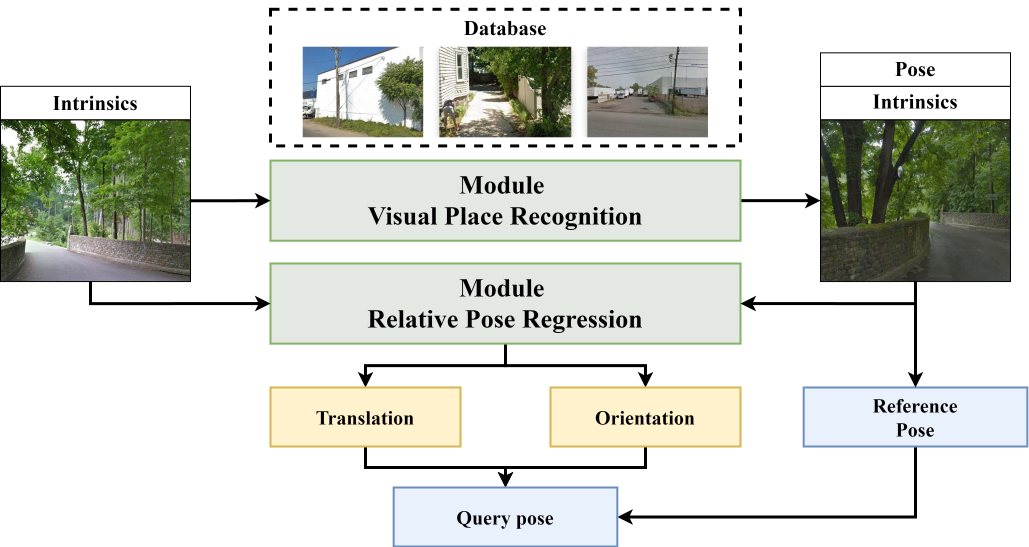
\includegraphics[width=\textwidth]{pics/Proposal/arch.png}
    % \includesvg[scale=0.3]{pics/Proposal/arch.svg}
    \caption{Kiến trúc tổng quan của pipeline định vị trực quan được đề xuất}
    \label{fig:arch}
\end{figure}

Gọi $I$ là ảnh mà người dùng chụp từ camera và được dùng làm ảnh truy vấn cho pipeline đề xuất của chúng tôi. Trước hết, pipeline nhận $I$ làm đầu vào cho MixVPR. Từ ảnh đầu vào $I$, sau khi qua các giai đoạn xử lý, MixVPR trả về một đoạn mã hóa biểu diễn cho nội dung của ảnh. Với đoạn mã hóa này, pipeline tiến hành so sánh với giá trị mã hóa của các ảnh trong cơ sở dữ liệu và tìm ra ảnh có sự tương đồng cao nhất với ảnh nhận vào $I$ gọi là $I_0$.

Bước tiếp theo, pipeline tiếp tục truyền cả ảnh nhận vào $I$ và ảnh được truy xuất $I_0$ cho mô hình tương quan 2D - 2D của Map-free Relocalization \cite{arnold2022mapfree}. Với đầu vào là cặp ảnh $(I, I_0)$, những cặp đặc trưng tương quan giữa hai ảnh được xác định tương ứng với mỗi hình. Sau đó, Essential Matrix $E$ giữa 2 ảnh được ước tính. Essential Matrix sau đó được phân giải thành ma trận thể hiện góc quay chênh lệch $R$ và một vector đơn vị độ dịch vị trí $\hat{t}$. Từ các cặp đặc trưng và độ sâu của ảnh, mô hình tiến hành một bước chiếu 3D để tính toán giá trị tỷ lệ $s$ của vector độ dịch vị trí. Cuối cùng, tư thế thực của camera được xác định bằng tư thế thực của ảnh tham khảo và độ lệch giữa ảnh tham khảo và ảnh truy vấn $(R,s*\hat{t})$.

\subsection{Dữ liệu đầu vào và đầu ra}
Mô hình nhận vào ảnh $I$, có định dạng là một ảnh RGB. Sau đó, ảnh $I$ được tiền xử lý, gồm các bước đưa về kích thước 320x320 và chuẩn hóa các điểm ảnh trên hình, trước khi được đưa vào mô hình chính. Lưu ý, mô hình kết hợp cần ảnh phải mang thông tin tham số nội tại của máy ảnh nhằm thực hiện bước hồi quy tư thế.

Qua quá trình mô phỏng lại bài toán nhận diện địa điểm trực quan, mô hình thu được $k$ cặp ảnh có độ tương đồng cao, gồm ảnh truy vấn ban đầu và ảnh tham khảo truy xuất được. Từng cặp ảnh trong $k$ cặp này được đưa vào bộ phận hồi quy tư thế tương đối tiếp theo. Có được tư thế của ảnh $I$ so với $k$ ảnh tham khảo có độ tương đồng cao nhất, mô hình chọn ra kết quả cuối cùng dựa vào độ đáng tin cậy $C$ được xác định ở \textbf{bộ phận xác định Essential Matrix}.

Định dạng đầu ra của mô hình gồm hai tập vector $R$ và $t$, lần lượt thể hiện góc quay và vị trí chụp ảnh trong không gian 3D. Cụ thể, hai vector có dạng:
\begin{itemize}
    \item \textbf{Vector góc quay $R$} có định dạng của một Quaternion, gồm 4 số là $(q_w, q_x, q_y, q_z)$. Quaternion có thể được dùng để biểu diễn góc quay trong không gian 3D và có thể dùng để thay thế ma trận xoay 3x3, nhằm có thể thể hiện và kết hợp các phép quay một cách dễ dàng hơn. Công thức biểu diễn một góc quay là
          \begin{equation}
              q=q_w + i*q_x + j*q_y + k*q_z,
          \end{equation}
          với $q_w, q_x, q_y, q_z$ là các số thực với $i,j,k$ là những vector đơn vị trực giao lẫn nhau. Quaternion có thể được biến đổi theo dạng trục quay và góc quay, có thể được biểu diễn bởi hai thành phần là vector đơn vị biểu diễn trục của góc quay, $(\hat{x},\hat{y},\hat{z})$ và độ quay quanh trục, $\theta$.
          \begin{figure}[H]
              \centering
              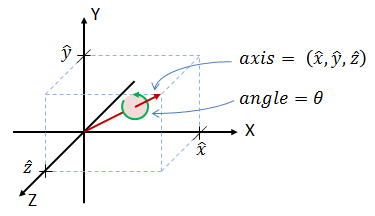
\includegraphics[scale=1]{pics/Proposal/axis-angle.png}
              \caption{Minh họa cách biểu diễn trục quay và góc quay \cite{quaternion}}
          \end{figure}
          Quaternion có thể được ước tính từ cách biểu diễn trục quay và góc quay theo công thức
          \begin{equation}
              \begin{aligned}
                   & q_w=\cos \left(\frac{\theta}{2}\right)          \\
                   & q_x=\hat{x} \sin \left(\frac{\theta}{2}\right)  \\
                   & q_y=\hat{y} \sin \left(\frac{\theta}{2}\right)  \\
                   & q_z=\hat{z} \sin \left(\frac{\theta}{2}\right),
              \end{aligned}
          \end{equation}
          với tập các giá trị $q_w, q_x, q_y, q_z$ có độ lớn là 1, dẫn đến tập các giá trị này có 3 độ tự do, 3DoF.
    \item \textbf{Vector vị trí $t$} có 3 giá trị là $t_x,t_y,t_z$ lần lượt thể hiện các giá trị kinh độ, vĩ độ và độ cao của vị trí chụp ảnh trong không gian thực tế. Vector thể hiện vị trí có cách biểu diễn đơn giản và dễ hiểu hơn so với góc quay. Ngoài ra, do biểu diễn không gian 3D thực tế nên vector thể hiện vị trí có 3 độ tự do.
\end{itemize}

\section{Module nhận diện địa điểm trực quan - VPR}
Module VPR của pipeline được phát triển dựa trên mô hình MixVPR được giới thiệu trong bài \cite{alibey2023mixvpr}. Đây là một phương pháp tổng hợp đặc trưng. Từ kết quả đặc trưng xác định được từ mô hình backbone, MixVPR giới thiệu một phương pháp tổng hợp mới, được thực hiện bởi khối Feature Mixer, một cấu trúc đặc biệt được xây dựng dựa trên mô hình MLP-Mixer \cite{tolstikhin2021mlpmixer}. Mô hình MixVPR sử dụng những khối này nhằm tích hợp thông tin toàn cục vào các đặc trưng. Nhờ vào kiến trúc nhẹ của khối Feature Mixer, hướng tiếp cận này cho phép MixVPR đạt hiệu năng cao ở tập dữ liệu thành thị phạm vi rộng mà không có tác động tài nguyên lớn.

\subsection{Kiến trúc}

\begin{figure}[H]
    \centering
    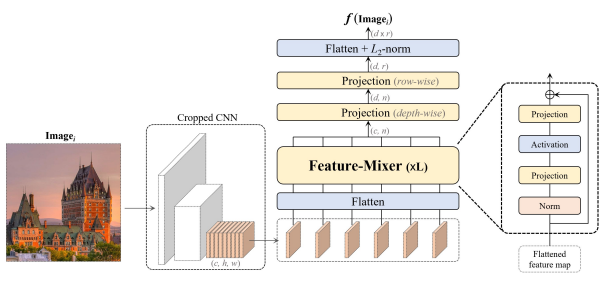
\includegraphics[width=\textwidth]{pics/Proposal/mixvpr.png}
    \caption{Tổng quan quá trình hoạt động của MixVPR \cite{alibey2023mixvpr}}
\end{figure}

\subsubsection{Mô hình backbone trích xuất đặc trưng thô}
Khi ảnh truy vấn $I$ được đưa vào, mô hình CNN backbone được sử dụng để trích xuất ra những chi tiết mang thông tin cần thiết. Mô hình cơ sở được huấn luyện trên những tập dữ liệu hình ảnh đa dạng, nhằm có thể phát hiện ra những đặc trưng quan trọng phục vụ các tác vụ liên quan đến thị giác máy tính. Trong kiến trúc đề xuất, mô hình cơ sở được cắt ở giữa, nhằm thu được tập những bản đồ đặc trưng $F$ có định dạng $F \in R^{c \cdot h \cdot w}$.

Ở những phương pháp trước đây như NetVLAD \cite{arandjelovic2016netvlad} và PatchNetVLAD \cite{hausler2021patchnetvlad}, những lớp bản đồ đặc trưng thuộc $F$ được xem như là một mô tả tương ứng với một miền tiếp nhận cho một khu vực trong ảnh ban đầu. Ngược lại, MixVPR xem $F$ như một tập các bản đồ đặc trưng 2D có kích thước $h \cdot w$, miêu tả toàn ảnh. Đây là một cách biểu diễn ảnh nhỏ, nhẹ và thống nhất hơn trong điều kiện thay đổi về ánh sáng và góc nhìn, thay cho việc lưu trữ từng điểm ảnh.
\begin{equation}
    F = \{X^{i}\},
\end{equation}
với $i \in \left[1,..,c\right]$ và $X^{i}$ tương ứng với bản đồ kích hoạt thứ $i$ ở F.

Mỗi bản đồ đặc trưng $X^{i}$ thuộc tập $F$ sau đó được được định dạng lại thành ma trận một chiều có dạng $X_{flat}^{i} \in R^{h*w}$, thu được được $F_{flat} \in R^{c \cdot n}$ với $n = h*w$.

\subsubsection{Khối tổng hợp Feature Mixer}
Tiếp theo, tập hợp của những bản đồ đặc trưng $F_{flat}$ lần lượt được đưa qua $L$ khối Feature Mixer, được phát triển trên cấu trúc mạng MLP. Mỗi khối Feature Mixer nhận vào từng bản đồ đặc trưng $X_{flat}^{i}$ một chiều và tích hợp thông tin về mối liên kết giữa các giá trị của $X_{flat}^{i}$ lên chính nó thông qua cách sau:
\begin{equation}
    \begin{aligned}
        X^{i} & \leftarrow Norm(X^{i})             \\
        X^{i} & \leftarrow W_2(\sigma(W_1 X^{i})),
    \end{aligned}
\end{equation}
với $W_1$ và $W_2$ là trọng số của hai lớp liên kết đầy đủ, cấu tạo nên MLP và $\sigma$ là hàm tạo sự phi tuyến tính cho quá trình xử lý (ReLU). Kỹ thuật nối tắt được sử dụng để nối đầu vào đã qua lớp chuẩn hóa với đầu ra nhằm giúp độ dốc trong quá trình huấn luyện có thể được truyền tải dễ hơn, cải thiện quá trình huấn luyện. Kết quả đầu ra của khối Feature Mixer được giữ định dạng giống như dữ liệu đầu vào, có dạng $R^{h*w}$.

Mục đích của việc sử dụng Feature Mixer là để tận dụng khả năng tổng hợp thông tin từ dữ liệu của các lớp kết nối đầy đủ, thay vì học trên những đặc trưng cục bộ trên ảnh và sử dụng cơ chế tập trung. Ngoài ra, Feature Mixer cũng trả về kết quả có định dạng và kích thước như đầu vào, thay vì giảm dần như những phương pháp tổng hợp dạng phân cấp (kim tự tháp) như trước đây, để mỗi neuron đều có thể biết được thông tin của toàn bộ ảnh. Những lớp MLP trong khối Feature Mixer giúp tích hợp thông tin trên toàn bộ ảnh qua mỗi lần xử lý.

Mỗi khối Feature Mixer sau khi xử lý xong từng bản đồ đặc trưng trong tập $F_{flat} \in R^{c \cdot n}$ ghép kết quả lại, tạo thành $Z \in R^{c \cdot n}$ với cùng kích thước trước khi được đưa vào khối Feature Mixer kế tiếp. Quá trình xử lý tập bản đồ đặc trưng qua các khối Feature Mixer có thể được miêu tả bằng công thức sau:
\begin{equation}
    Z = FM_L(FM_{L-1}(\dots FM_1(F_{flat}))),
\end{equation}
với $FM_i$ là lớp Feature Mixer thứ $i$ trên tổng số $L$ khối và $Z$ là kết quả cuối cùng của quá trình tích hợp thông tin toàn cục.

\subsubsection{Lớp tổng hợp - Aggregation}
Ta có $Z \in R^{c \cdot n}$ với số chiều rất cao do có định dạng được giữ nguyên so với $F_{flat}$. Để giúp giảm bớt số chiều của $Z$ lại sau khi qua khối Feature Mixer, hai lớp kết nối đầy đủ được sử dụng để thực hiện tác vụ tổng hợp lần lượt giữa các giá trị trên cùng một kênh $c$ với nhau và sau đó là giữa các giá trị trong từng bản đồ đặc trưng $X_{flat}^i$. Tác vụ này thực hiện việc tổng hợp có chọn lọc nhằm điều khiển được kích thước của giá trị đầu ra.

Đầu tiên, dữ liệu được tổng hợp số kênh để biến định dạng của $Z$ từ $R^{c \cdot n}$ thành $R^{d \cdot n}$.
\begin{equation}
    Z' = W_d(Transpose(Z)),
\end{equation}
với $W_d$ là trọng số của lớp kết nối đầy đủ đầu tiên và $d$ là định dạng đầu ra sau khi rút gọn số kênh lại, $d<c$.

Sau đó, giá trị trên từng bản đồ đặc trưng được tổng hợp lại, từ định dạng $R^{d \cdot n}$ thành $R^{d \cdot r}$.
\begin{equation}
    O = W_r(Transpose(Z')),
\end{equation}
với $W_r$ là trọng số của lớp kết nối đầy đủ thứ hai và $r$ là định dạng đầu ra của các bản đồ đặc trưng 1D, $r<n$.

Kết quả $O$ cuối cùng, có định dạng là $R^{d \cdot r}$, được ép thành một chiều và chuẩn hóa theo $L_2$ như những phương pháp VPR khác \cite{arandjelovic2016netvlad,berton2022rethinking}. Cuối cùng, từ ảnh đầu vào $I$, mô hình trả về một đoạn mã hóa biểu diễn cho nội dung của ảnh. Đoạn mã hóa này sau đó có thể được dùng để so sánh với giá trị mã hóa của những hình khác nhằm tìm ảnh có độ tương đồng cao nhất với $I$.

\subsubsection{Bộ phận truy vấn ảnh tương đồng}
Sau khi đã có được giá trị mã hóa biễu diễn cho ảnh truy vấn là $O \in R^{d \cdot r}$, mô hình tiến hành tìm kiếm trên tập dữ liệu ảnh miêu tả khu vực đang xét. Cơ chế tìm kiếm được sử dụng là tìm kiếm toàn diện, xét giá trị biểu diễn của từng ảnh. $k$ ảnh có độ tương đồng cao nhất với ảnh truy vấn được chọn để tạo thành các cặp ảnh là đầu ra của bước này.

\begin{figure}[H]
    \centering
    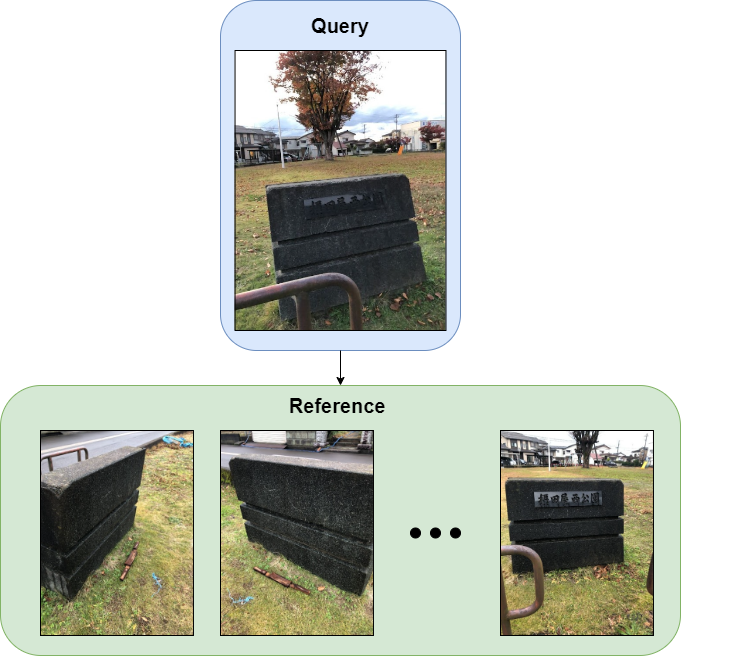
\includegraphics[scale=0.4]{pics/Proposal/query.png}
    \caption[Kết quả của module VPR]{Ảnh truy xuất được từ ảnh truy vấn $I$ ban đầu, từ tập dữ liệu Niantic \cite{arnold2022mapfree}}
\end{figure}


\subsection{Phương pháp hiện thực và triển khai}

\subsubsection{Hiện thực}

Mô hình MixVPR được hiện thực trên framework PyTorch. Mô hình CNN cơ sở của MixVPR được cắt ở lớp áp cuối của mô hình ResNet. Dữ liệu đầu vào cho MixVPR là các ảnh đã được chỉnh về độ phân giải $320x320$ và qua mô hình backbone, một tập các bản đồ đặc trưng có kích thước 20x20 được đưa vào tập $L$ khối Feature Mixer. Thao tác tổng hợp trong khối Feature Mixer sử dụng lớp Linear, theo sau đó là một lớp ReLU để tạo tính phi tuyến tính. Về lớp chuẩn hóa, LayerNorm được sử dụng. Cuối cùng, đầu ra cuối cùng của khối Feature Mixer được tổng hợp xuống một chiều không gian biểu diễn nhỏ hơn sử dụng hai lớp kết nối đầy đủ giữa các kênh với nhau và giữa các giá trị trong mỗi kênh, chứng minh rằng MixVPR là một cấu trúc chỉ sử dụng MLP. Số khối Feature Mixer được sử dụng mặc định là $L=4$.

\subsubsection{Huấn luyện}
Mô hình MixVPR được đánh giá trong bài nghiên cứu sử dụng mô hình ResNet \cite{he2016deep} đã được huấn luyện trên tập ImageNet \cite{krizhevsky2012imagenet} làm cơ sở. Sau đó, mô hình được huấn luyện trên tập dữ liệu GSV-Cities \cite{Ali_bey_2022}. Đối với hàm mất mát, hàm Multi-Similarity Loss \cite{wang2019multi} được sử dụng với lý do đã được chứng minh là hỗ trợ cho ra kết quả tốt nhất với tác vụ VPR \cite{Ali_bey_2022}. Kích thước của một batch có $P = 120$ địa điểm, mỗi địa điểm được miêu tả bởi 4 ảnh, tạo thành một batch có kích thước 480 ảnh. Phương pháp tối ưu giảm độ dốc ngẫu nhiên - SGD được sử dụng với quán tính - momentum là 0.9 với giá trị suy giảm trọng số - weight decay là 0.001. Tốc độ học - learning rate được khởi tạo với giá trị 0.05 và được chia 3 sau mỗi 5 chu kỳ - epoch. Cuối cùng, mô hình được huấn luyện tối đa 30 chu kỳ - epoch với đầu vào là ảnh đã được điều chỉnh kích thước 320x320.

\subsubsection{Phương pháp đánh giá}
Để đánh giá hiệu năng mô hình, 5 tập dữ liệu tiêu chuẩn đã được sử dụng. Pitts250k-test \cite{6618963}, bao gồm 8.000 ảnh truy vấn và 83.000 ảnh tham khảo, được thu thập từ Google Street View và Pitts30k-test \cite{6618963} là một tập con của Pitts250k bao gồm 8.000 ảnh truy vấn và 8.000 ảnh tham khảo. Cả 2 tập dữ liệu Pittsburgh đều có những góc nhìn có độ lệch đáng kể, những chi tiết kiến trúc tương đồng cũng thường xuyên xuất hiện trong tập dữ liệu này. Tập dữ liệu SPEDTest \cite{zaffar2021vpr} gồm 607 ảnh truy vấn và 607 ảnh tham khảo thu từ camera giám sát, chứa những thay đổi lớn về độ sáng và về cảnh vật các mùa. MSLS \cite{warburg2020mapillary} được thu thập từ camera hành trình của xe hơi, cho rất nhiều góc nhìn đa dạng cũng như đa dạng về sự thay đổi độ sáng. Cuối cùng, Nordland \cite{zaffar2021vpr} là một tập dữ liệu chứa nhiều thử thách khi sử dụng ảnh thu thập được ở cả 4 mùa với camera được gắn trên tàu. Đơn vị đánh giá được sử dụng là recall@k, thể hiện tỷ lệ của truy xuất thành công trên tổng số lượng truy xuất. Một truy xuất hình được xem là thành công khi ảnh được truy xuất nằm trong vòng 25m xung quanh ảnh truy vấn.

\subsection{Kết quả}
Khi so sánh trên những tập dữ liệu phản ánh môi trường thành thị, mô hình MixVPR đạt được kết quả vượt trội so với những mô hình SOTA đã được đề xuất trước nó, như CosPlace \cite{berton2022rethinking} và NetVLAD \cite{arandjelovic2016netvlad}. Những tập dữ liệu được sử dụng đã bao quát hết những trường hợp có thể tác động xấu đến mô hình như góc nhìn đa dạng; thời tiết, mùa thay đổi; chênh lệch về độ sáng. MixVPR cũng có khả năng giải quyết được những trường hợp mà những phương pháp trước gặp khó khăn như: kiến trúc lặp lại nhiều, góc nhìn thay đổi rõ rệt, đường chân trời, độ sáng chênh lệch lớn và gặp nhiều vật thể cản trở tầm nhìn. Tuy nhiên, mô hình vẫn gặp thất bại khi độ chênh lệch góc nhìn là quá lớn hoặc có quá nhiều vật cản. Những trường hợp thất bại của mô hình MixVPR được thể hiện ở hình \textbf{3.5}

\begin{figure}
    \centering
    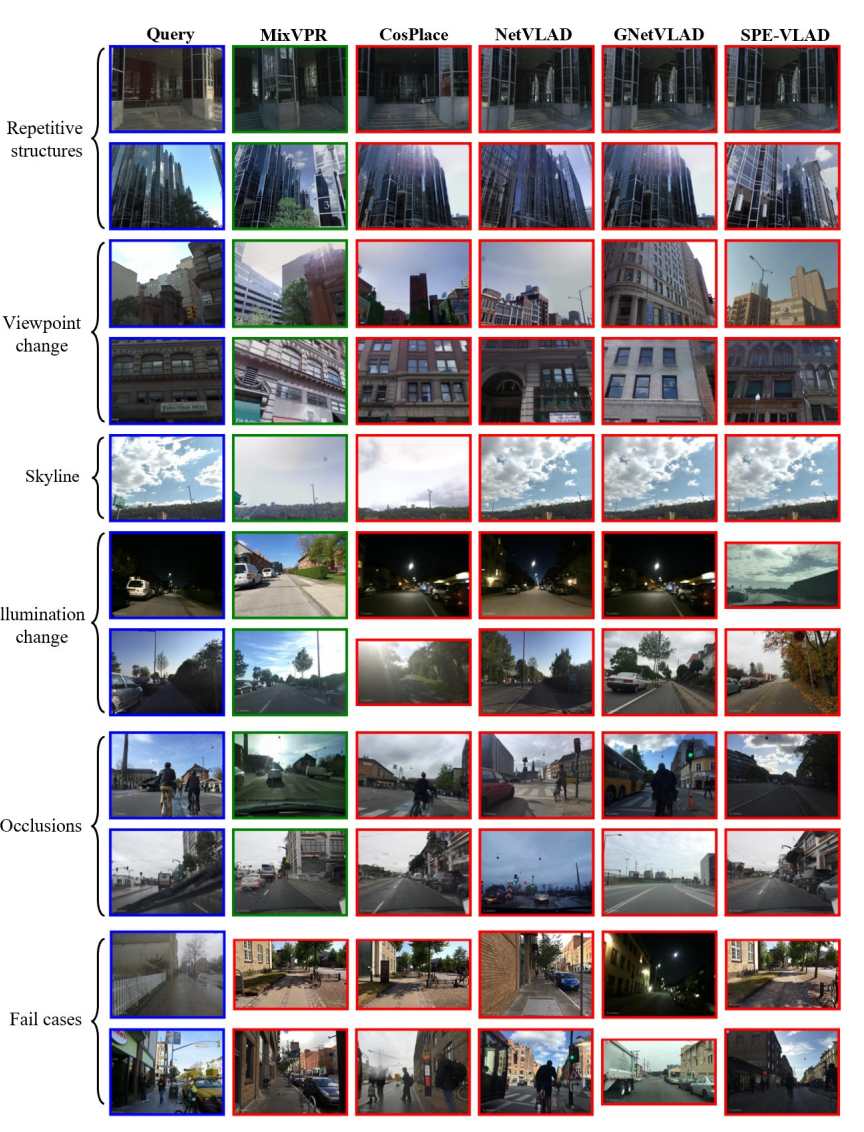
\includegraphics[width=\textwidth]{pics/Proposal/fail.png}
    \caption{Kết quả của những trường hợp khó khi chạy trên MixVPR và các phương pháp khác \cite{alibey2023mixvpr}}
\end{figure}

Với sự ra đời của AnyLoc \cite{keetha2023anyloc}, bài toán VPR trong những môi trường đa dạng hơn như trong nhà, trong hang động, trên bầu trời, hoặc trên mặt biển đã có một SOTA mới. Điều này là nhờ việc AnyLoc sử dụng mạng cơ sở DINO, một mạng Vision Transformer được huấn luyện bằng cơ chế tự giám sát để sinh ra những đặc trưng có giá trị với mọi tác vụ. Tuy nhiên, khi xét đến môi trường thành thị thì MixVPR vẫn có cho ra kết quả chính xác hơn AnyLoc. Số liệu cụ thể được trình bày bên dưới.

% \begin{figure}[H]
%   \centering
%   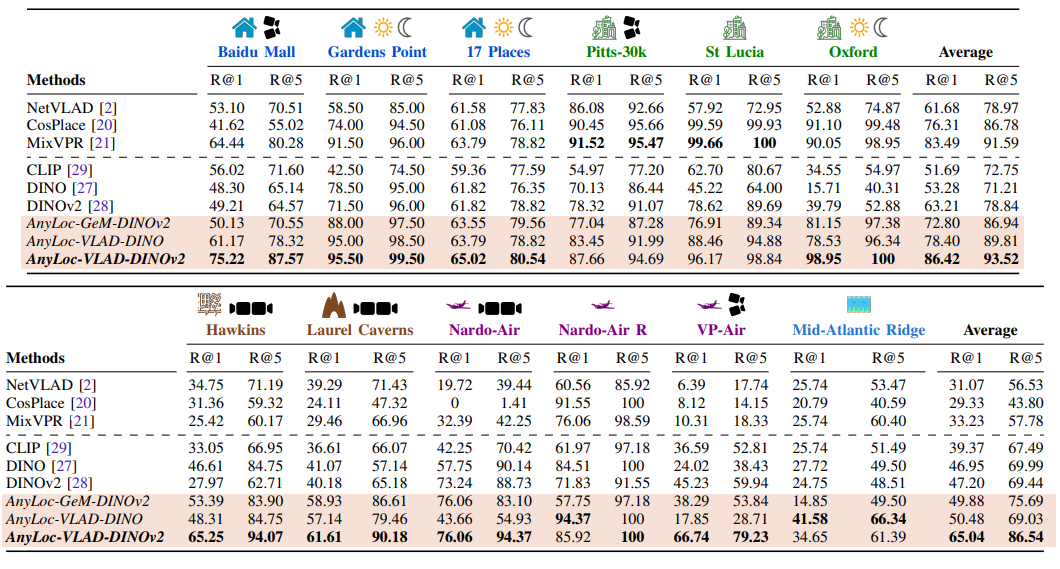
\includegraphics[scale=0.5]{pics/Proposal/anyloc.png}
%   \caption{Kết quả của AnyLoc so sánh với những mô hình khác \cite{keetha2023anyloc}}
% \end{figure}


\begin{table}[H]
    \adjustbox{max width=\textwidth}{
        \begin{tabular}{lcccccccccccccc}
            \cline{2-15}
            \multicolumn{1}{l|}{}                  & \multicolumn{2}{c|}{{\color[HTML]{6434FC} \textbf{Baidu Mall}}} & \multicolumn{2}{c|}{{\color[HTML]{6434FC} \textbf{Gardens Point}}} & \multicolumn{2}{c|}{{\color[HTML]{6434FC} \textbf{17 Places}}} & \multicolumn{2}{c|}{{\color[HTML]{009901} \textbf{Pitts-30k}}} & \multicolumn{2}{c|}{{\color[HTML]{009901} \textbf{St Lucia}}} & \multicolumn{2}{c|}{{\color[HTML]{009901} \textbf{Oxford}}} & \multicolumn{2}{c|}{\textbf{Average}}                                                                                                                                                                                              \\ \hline
            \multicolumn{1}{|l|}{\textbf{Methods}} & \multicolumn{1}{c|}{R@1}                                        & \multicolumn{1}{c|}{R@5}                                           & \multicolumn{1}{c|}{R@1}                                       & \multicolumn{1}{c|}{R@5}                                       & \multicolumn{1}{c|}{R@1}                                      & \multicolumn{1}{c|}{R@5}                                    & \multicolumn{1}{c|}{R@1}              & \multicolumn{1}{c|}{R@5} & \multicolumn{1}{c|}{R@1} & \multicolumn{1}{c|}{R@5} & \multicolumn{1}{c|}{R@1} & \multicolumn{1}{c|}{R@5} & \multicolumn{1}{c|}{R@1} & \multicolumn{1}{c|}{R@5} \\ \hline
            NetVLAD                                & 53.10                                                           & 70.51                                                              & 58.50                                                          & 85.00                                                          & 61.58                                                         & 77.83                                                       & 86.08                                 & 92.66                    & 57.92                    & 72.95                    & 52.88                    & 74.87                    & 61.68                    & 78.97                    \\
            CosPlace                               & 41.62                                                           & 55.02                                                              & 74.00                                                          & 94.50                                                          & 61.08                                                         & 76.11                                                       & 90.45                                 & 95.66                    & 99.59                    & 99.93                    & 91.10                    & 99.48                    & 76.31                    & 86.78                    \\
            MixVPR                                 & 64.44                                                           & 80.28                                                              & 91.50                                                          & 96.00                                                          & 63.79                                                         & 78.82                                                       & \textbf{91.52}                        & \textbf{95.47}           & \textbf{99.66}           & \textbf{100}             & 90.05                    & 98.95                    & 83.49                    & 91.59                    \\ \hline
            CLIP                                   & 56.02                                                           & 71.60                                                              & 42.50                                                          & 74.50                                                          & 59.36                                                         & 77.59                                                       & 54.97                                 & 77.20                    & 62.70                    & 80.67                    & 34.55                    & 54.97                    & 51.69                    & 72.75                    \\
            DINO                                   & 48.30                                                           & 65.14                                                              & 78.50                                                          & 95.00                                                          & 61.82                                                         & 76.35                                                       & 70.13                                 & 86.44                    & 45.22                    & 64.00                    & 15.71                    & 40.31                    & 53.28                    & 71.21                    \\
            DINOv2                                 & 49.21                                                           & 64.57                                                              & 71.50                                                          & 96.00                                                          & 61.82                                                         & 78.82                                                       & 78.32                                 & 91.07                    & 78.62                    & 89.69                    & 39.79                    & 52.88                    & 63.21                    & 78.84                    \\
            \rowcolor[HTML]{FFCE93}
            \textit{AnyLoc-GeM-DINOv2}             & 50.13                                                           & 70.55                                                              & 88.00                                                          & 97.50                                                          & 63.55                                                         & 79.56                                                       & 77.04                                 & 87.28                    & 76.91                    & 89.34                    & 81.15                    & 97.38                    & 72.80                    & 86.94                    \\
            \rowcolor[HTML]{FFCE93}
            \textit{AnyLoc-VLAD-DINO}              & 61.17                                                           & 78.32                                                              & 95.00                                                          & 98.50                                                          & 63.79                                                         & 78.82                                                       & 83.45                                 & 91.99                    & 88.46                    & 94.88                    & 78.53                    & 96.34                    & 78.40                    & 89.81                    \\
            \rowcolor[HTML]{FFCE93}
            \textit{\textbf{AnyLoc-VLAD-DINOv2}}   & \textbf{75.22}                                                  & \textbf{87.57}                                                     & \textbf{95.50}                                                 & \textbf{99.50}                                                 & \textbf{65.02}                                                & \textbf{80.54}                                              & 87.66                                 & 94.69                    & 96.17                    & 98.84                    & \textbf{98.95}           & \textbf{100}             & \textbf{86.42}           & \textbf{93.52}
        \end{tabular}}
    \caption{Bảng so sánh kết quả AnyLoc với những mô hình khác trên những tập dữ liệu thành thị}
\end{table}

\begin{table}[H]
    \adjustbox{max width=\textwidth}{
        \begin{tabular}{lcccccccccccccc}
            \cline{2-15}
            \multicolumn{1}{l|}{}                  & \multicolumn{2}{c|}{{\color[HTML]{986536} \textbf{Hawkins}}} & \multicolumn{2}{c|}{{\color[HTML]{986536} \textbf{Laurel Caverns}}} & \multicolumn{2}{c|}{{\color[HTML]{6200C9} \textbf{Nardo-Air}}} & \multicolumn{2}{c|}{{\color[HTML]{6200C9} \textbf{Nardo-Air R}}} & \multicolumn{2}{c|}{{\color[HTML]{6200C9} \textbf{VP-Air}}} & \multicolumn{2}{c|}{{\color[HTML]{3531FF} \textbf{\begin{tabular}[c]{@{}c@{}}Mid-Atlantic\\ Ridge\end{tabular}}}} & \multicolumn{2}{c|}{\textbf{Average}}                                                                                                                                                                                              \\ \hline
            \multicolumn{1}{|l|}{\textbf{Methods}} & \multicolumn{1}{c|}{R@1}                                     & \multicolumn{1}{c|}{R@5}                                            & \multicolumn{1}{c|}{R@1}                                       & \multicolumn{1}{c|}{R@5}                                         & \multicolumn{1}{c|}{R@1}                                    & \multicolumn{1}{c|}{R@5}                                                                                          & \multicolumn{1}{c|}{R@1}              & \multicolumn{1}{c|}{R@5} & \multicolumn{1}{c|}{R@1} & \multicolumn{1}{c|}{R@5} & \multicolumn{1}{c|}{R@1} & \multicolumn{1}{c|}{R@5} & \multicolumn{1}{c|}{R@1} & \multicolumn{1}{c|}{R@5} \\ \hline
            NetVLAD                                & 34.75                                                        & 71.19                                                               & 39.29                                                          & 71.43                                                            & 19.72                                                       & 39.44                                                                                                             & 60.56                                 & 85.92                    & 6.39                     & 17.74                    & 25.74                    & 53.47                    & 31.07                    & 56.53                    \\
            CosPlace                               & 31.36                                                        & 59.32                                                               & 24.11                                                          & 47.32                                                            & 0                                                           & 1.41                                                                                                              & 91.55                                 & \textbf{100}             & 8.12                     & 14.15                    & 20.79                    & 40.59                    & 29.33                    & 43.80                    \\
            MixVPR                                 & 25.42                                                        & 60.17                                                               & 29.46                                                          & 66.96                                                            & 32.39                                                       & 42.25                                                                                                             & 76.06                                 & 98.59                    & 10.31                    & 18.33                    & 25.74                    & 60.40                    & 33.23                    & 57.78                    \\ \hline
            CLIP                                   & 33.05                                                        & 66.95                                                               & 36.61                                                          & 66.07                                                            & 42.25                                                       & 70.42                                                                                                             & 61.97                                 & 97.18                    & 36.59                    & 52.81                    & 25.74                    & 51.49                    & 39.37                    & 67.49                    \\
            DINO                                   & 46.61                                                        & 84.75                                                               & 41.07                                                          & 57.14                                                            & 57.75                                                       & 90.14                                                                                                             & 84.51                                 & 100                      & 24.02                    & 38.43                    & 27.72                    & 49.50                    & 46.95                    & 69.99                    \\
            DINOv2                                 & 27.97                                                        & 62.71                                                               & 40.18                                                          & 65.18                                                            & 73.24                                                       & 88.73                                                                                                             & 71.83                                 & 91.55                    & 45.23                    & 59.94                    & 24.75                    & 48.51                    & 47.20                    & 69.44                    \\
            \rowcolor[HTML]{FFCE93}
            \textit{AnyLoc-GeM-DINOv2}             & 53.39                                                        & 83.90                                                               & 58.93                                                          & 86.61                                                            & 76.06                                                       & 83.10                                                                                                             & 57.75                                 & 97.18                    & 38.29                    & 53.84                    & 14.85                    & 49.50                    & 49.88                    & 75.69                    \\
            \rowcolor[HTML]{FFCE93}
            \textit{AnyLoc-VLAD-DINO}              & 48.31                                                        & 84.75                                                               & 57.14                                                          & 79.46                                                            & 43.66                                                       & 54.93                                                                                                             & \textbf{94.37}                        & \textbf{100}             & 17.85                    & 28.71                    & \textbf{41.58}           & \textbf{66.34}           & 50.48                    & 69.03                    \\
            \rowcolor[HTML]{FFCE93}
            \textit{\textbf{AnyLoc-VLAD-DINOv2}}   & \textbf{65.25}                                               & \textbf{94.07}                                                      & \textbf{61.61}                                                 & \textbf{90.18}                                                   & \textbf{76.06}                                              & \textbf{94.37}                                                                                                    & 85.92                                 & \textbf{100}             & \textbf{66.74}           & \textbf{79.23}           & 34.65                    & 61.39                    & \textbf{65.04}           & \textbf{86.54}
        \end{tabular}}
    \caption{Bảng so sánh kết quả AnyLoc với những mô hình khác trên những tập dữ liệu ngoài thiên nhiên}
\end{table}
\section{Module hồi quy tư thế tương đối - RPR}
Mô hình tương quan 2D-2D được đề xuất trong Map-free Relocalization \cite{arnold2022mapfree} thuộc nhóm những phương pháp định vị theo hướng tiếp cận truyền thống sử dụng Essential Matrix. So với những phương pháp RPR thường thấy, phương pháp này giải quyết được vấn đề không nắm bắt được thông tin về hình học trong ảnh. Mô hình vẫn đạt được kết quả cạnh tranh trong những môi trường có mật độ ảnh dày đặc. Tuy nhiên, khi được đưa vào môi trường mà ảnh tham khảo và ảnh truy vấn xa nhau hơn thì phương pháp này lại có kết quả vượt trội hơn hẳn những phương pháp khác. Mô hình tương quan 2D-2D xác định Essential Matrix giữa 2 ảnh thông qua những cặp điểm tương quan, từ đó tính toán được khác biệt về hướng lệch vị trí và góc quay. Sử dụng thêm thông tin về độ sâu, mô hình xác định được khoảng cách cách biệt thực giữa cặp ảnh và qua đó có được vị trí thực của ảnh truy vấn.

\subsection{Kiến trúc}

\begin{figure}[htbp]
  \centering
  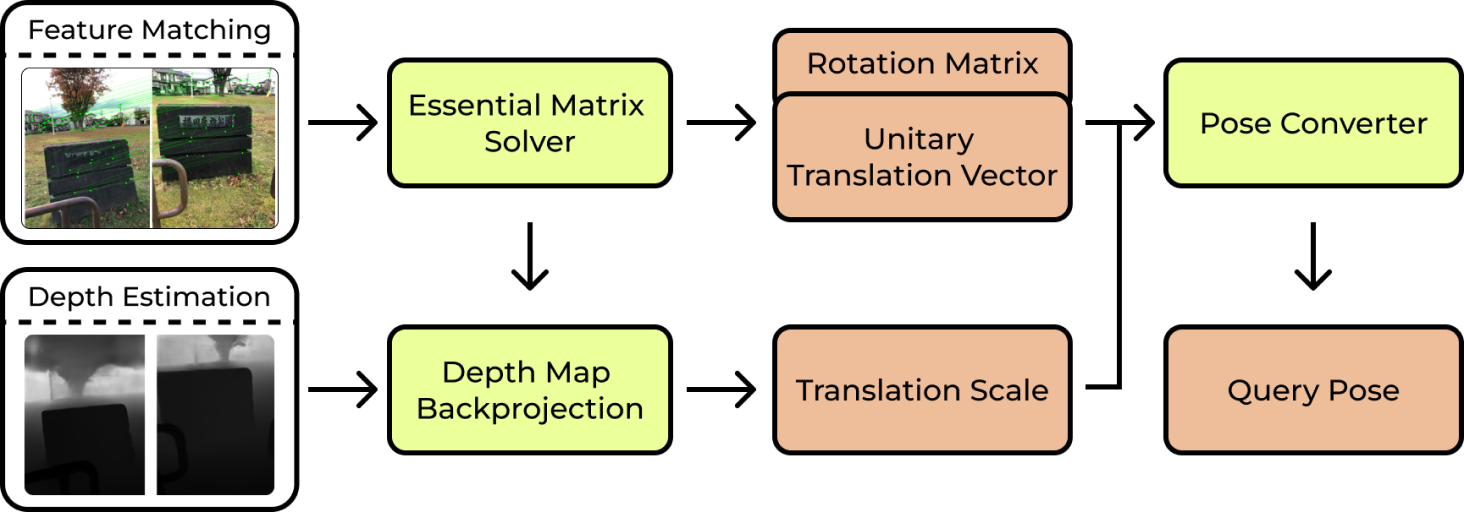
\includegraphics[width=\textwidth]{pics/Proposal/2d_2d.png}
  % \includesvg[scale=0.3]{pics/Proposal/arch.svg}
  \caption{Kiến trúc tổng quan của mô hình tương quan 2D-2D}
\end{figure}

\subsubsection{Mô hình xác định cặp đặc trưng và ước tính độ sâu của ảnh}

Với dữ liệu đầu vào là cặp ảnh gồm ảnh truy vấn và ảnh tham khảo $(I, I_0)$, tại bước này, những cặp đặc trưng tương quan sẽ được xác định và vị trí của chúng sẽ được lưu lại trong 2 tập là $(kpts_0, ktps_1)$. Mô hình ghép đặc trưng được sử dụng sẽ là SuperPoint+SuperGlue \cite{sarlin2020superglue} đã trải qua quá trình huấn luyện. Bản đồ thông tin độ sâu của mỗi ảnh cũng sẽ được sinh ra bằng mô hình DPT \cite{ranftl2021vision} được huấn luyện trên tập KITTI do phạm vi được sử dụng của mô hình sẽ là ở ngoài trời, trong khu vực thành thị \cite{arnold2022mapfree}. Dữ liệu trả về của 2 mô hình này sẽ là hai tập chứa vị trí của các điểm đặc trưng tương ứng và bản đồ độ sâu ước tính của mỗi hình.

\begin{figure}[H]
  \centering
  \begin{minipage}[b]{0.48\textwidth}
    \captionsetup{justification=centering}
    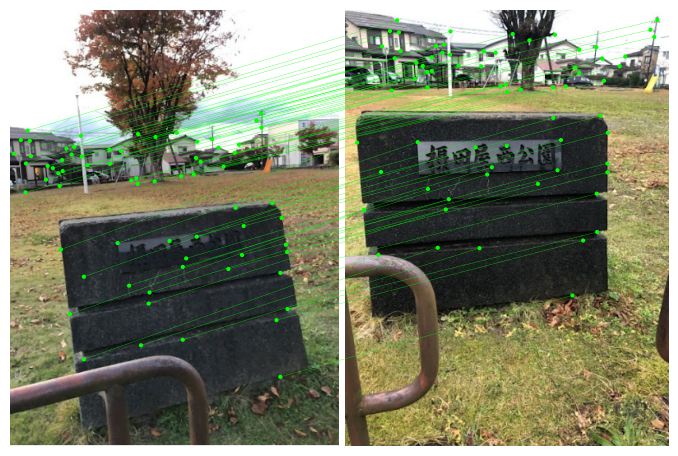
\includegraphics[width=\textwidth]{pics/Proposal/matching.png}
    \caption{Kết quả của quá trình xác định và ghép đặc trưng}
  \end{minipage}
  \begin{minipage}[b]{0.48\textwidth}
    \captionsetup{justification=centering}
    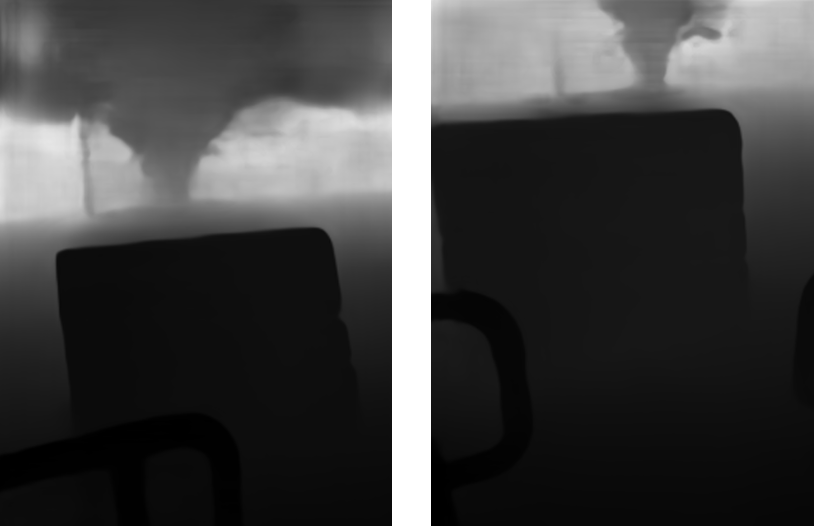
\includegraphics[width=\textwidth]{pics/Proposal/depth.png}
    \caption{Kết quả của quá trình ước tính độ sâu ảnh}
  \end{minipage}
  % \begin{minipage}[t]{0.3\textwidth}
  %     \caption{Kết quả của quá trình xác định và ghép đặc trưng}
  % \end{minipage}
  % \begin{minipage}[t]{0.3\textwidth}
  %     \caption{Kết quả của quá trình ước tính độ sâu ảnh}
  % \end{minipage}
\end{figure}

\subsubsection{Bộ phận khai phá Essential Matrix}

Dựa vào những cặp đặc trưng tương quan đã được xác định trong các tập $(kpts_0, kpts_1)$ và ma trận thông số $T_0, T_1$ của camera của mỗi ảnh, Essential Matrix $M$ được ước tính dựa vào giải thuật 5 điểm \cite{nister2004efficient} cùng với vòng lặp MAGSAC++ \cite{barath2020magsac++}. Ma trận thông số $T_i$ của camera sẽ chứa các thông tin về tiêu cự của camera $f_x,f_y$ và tọa độ điểm chính của camera $c_x,c_y$, được sắp xếp thành ma trận như sau:
\begin{equation}
  T_i = \begin{bmatrix} f_x & 0 & c_x \\ 0 & f_y & c_y \\ 0 & 0 & 1 \end{bmatrix}
\end{equation}
Essential Matrix $M$ sau đó sẽ được phân giải thành ma trận thể hiện góc quay chênh lệch, $R \in SO(3)$ và vector đơn vị độ lệch về vị trí giữa hai ảnh, $\hat{t} \in R^{3}, \lvert \hat{t} \rvert = 1$. Tập những cặp điểm tương quan thỏa Essential Matrix $M$ cũng sẽ được trả về.

\subsubsection{Bộ phận chiếu cặp điểm tương quan lên không gian ba chiều}

Những cặp điểm tương quan (inlier correspondence) thỏa ma trận $M$ sau đó sẽ được chiếu lên không gian 3D qua bản đồ độ sâu ảnh đã được sinh ra ở mỗi ảnh. Với mỗi cặp điểm $p_0, p_1$ đã được chiếu lên không gian 3D, mô hình sẽ tìm được một giá trị tỷ lệ $s^*$ cho $\hat{t}$ để làm giảm thiểu độ lệch của điểm $p_0$ khi được chiếu lên hệ tọa độ của camera thứ hai và điểm $p_1$. Giá trị $s$ tương ứng với mỗi cặp điểm $(p_0, p_1)$ có thể được xác định qua công thức:

\begin{equation}
  \begin{aligned}
    s=\underset{s^*}{\arg \min }\left\|R p_A+s^* \cdot \hat{t}-p_B\right\|_2 .
  \end{aligned}
\end{equation}

\begin{figure}[H]
  \centering
  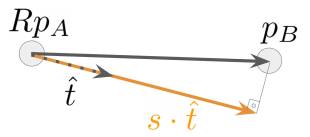
\includegraphics[scale=1]{pics/Proposal/reprojection.png}
  \caption[Minh họa cho việc xác định tỷ lệ $s$ bằng độ sâu ảnh]{Hình minh họa cho việc chiếu điểm $p_0$ qua vector góc quay $R$ và vector độ lệch đơn vị $\hat{t}$ cùng với tỷ lệ $s$ để tối thiểu khoảng cách \cite{arnold2022mapfree}}
\end{figure}

Cuối cùng, tỷ lệ $s^*$ với số cặp điểm hợp lệ cao nhất sẽ được chọn làm kết quả cuối cùng. Một cặp điểm sẽ được xem như hợp lệ khi khoảng cách sai lệch giữa hai điểm 3D sau khi chiếu nhỏ hơn một ngưỡng nhất định, ở đây được xác định là 10cm. Vòng lặp RANSAC sẽ được sử dụng để bỏ những trường hợp ngoại lệ.

Sau khi chạy qua những bước trên, mô hình sẽ thu về được các giá trị thể hiện độ lệch giữa vị trí và góc quay của cặp ảnh truy vấn và tham khảo dưới dạng ma trận độ lệch góc quay $R$ và vector độ lệch vị trí $s*\hat{t}$. Ma trận độ lệch góc quay $R$ sau đó sẽ được phân giải thành một Quaternion - được biểu diễn dưới dạng một tập 4 số là $q^{\Delta} = (q^{\Delta}_w,q^{\Delta}_x,q^{\Delta}_y,q^{\Delta}_z)$ - thể hiện góc quay trong không gian. Vector độ lệch vị trí sẽ có dạng bộ 3 số là $(t^{\Delta} = t^{\Delta}_x,t^{\Delta}_y,t^{\Delta}_z)$. Ngoài ra, số cặp điểm tương quan có độ lệch dưới 10cm với giá trị $s^*$ được chọn sẽ được dùng làm thông số đánh giá độ đáng tin cậy $C$ của dự đoán.


\subsubsection{Bộ phận tính toán tư thế tuyệt đối}

Từ kết quả của những bộ phận trên, mô hình đã biểu diễn được góc quay và vị trí tương đối giữa hai ảnh $(q^{\Delta},t^{\Delta})$. Khi biết được tọa độ chính xác của ảnh tham khảo $(q^{ref},t^{ref})$, mô hình sẽ tính được tọa độ và góc quay chính xác của ảnh truy vấn và đưa ra kết quả cuối cùng là hai tập $(q^{abs},t^{abs})$

Để xác định được góc quay chính xác của ảnh truy vấn, mô hình biến đổi góc quay của ảnh tham khảo với độ lệch góc quay đã xác định được giữa hai ảnh theo công thức:

\begin{equation}
  \begin{aligned}
    q^{abs}                                   & = q^{\Delta} * q^{ref}                                                                                    \\
    (q^{abs}_w,q^{abs}_x,q^{abs}_y,q^{abs}_z) & = (q^{\Delta}_w,q^{\Delta}_x,q^{\Delta}_y,q^{\Delta}_z) * (q^{ref}_w,q^{ref}_x,q^{ref}_y,q^{ref}_z)       \\ \\
    q^{abs}_w                                 & =\left(q^{\Delta}_w q^{ref}_w-q^{\Delta}_x q^{ref}_x-q^{\Delta}_y q^{ref}_y-q^{\Delta}_z q^{ref}_z\right) \\
    q^{abs}_x                                 & =\left(q^{\Delta}_w q^{ref}_x+q^{\Delta}_x q^{ref}_w-q^{\Delta}_y q^{ref}_z+q^{\Delta}_z q^{ref}_y\right) \\
    q^{abs}_y                                 & =\left(q^{\Delta}_w q^{ref}_y+q^{\Delta}_x q^{ref}_z+q^{\Delta}_y q^{ref}_w-q^{\Delta}_z q^{ref}_x\right) \\
    q^{abs}_z                                 & =\left(q^{\Delta}_w q^{ref}_z-q^{\Delta}_x q^{ref}_y+q^{\Delta}_y q^{ref}_x+q^{\Delta}_z q^{ref}_w\right)
  \end{aligned}
\end{equation}

Để xác định vị trí chính xác của ảnh truy vấn trong không gian thực, vị trí kinh độ, vĩ độ và độ cao của ảnh chụp có thể được xác định qua công thức:

\begin{equation}
  \begin{aligned}
    t^{abs}                         & = t^{\Delta} + t^{ref}                                                       \\
    (t^{abs}_x,t^{abs}_y,t^{abs}_z) & = (t^{\Delta}_x,t^{\Delta}_y,t^{\Delta}_z) + (t^{ref}_x,t^{ref}_y,t^{ref}_z) \\ \\
    t^{abs}_x                       & = t^{\Delta}_x + t^{ref}_x                                                   \\
    t^{abs}_y                       & = t^{\Delta}_y + t^{ref}_y                                                   \\
    t^{abs}_z                       & = t^{\Delta}_z + t^{ref}_z                                                   \\
  \end{aligned}
\end{equation}

\subsection{Phương pháp hiện thực và triển khai}
\subsubsection{Hiện thực}
Tác vụ tìm kiếm tương quan giữa hai ảnh có thể lựa chọn giữa các phương pháp truyền thống như SIFT, hoặc những phương pháp theo hướng tiếp cận học sâu gần đây như SuperPoint+SuperGlue \cite{sarlin2020superglue} và LoFTR \cite{sun2021loftr}. Tác vụ tính độ sâu đơn ảnh sẽ được phân thành hai trường hợp là bên trong nhà và ngoài trời. Với những tập dữ liệu trong nhà, mô hình DPT \cite{ranftl2021vision} được huấn luyện trên tập dữ liệu NYUv2 \cite{silberman2012indoor} PlaneRCNN \cite{liu2019planercnn} được huấn luyện trên tập dữ liệu ScanNet \cite{dai2017scannet}. Với trường hợp ngoài trời, mô hình DPT \cite{ranftl2021vision} được huấn luyện trên tập KITTI sẽ được sử dụng \cite{geiger2012we}. Mô hình SuperPoint+SuperGlue sẽ được chọn để thực hiện tác vụ Feature Matching và mô hình DPT được huấn luyện trên tập KITTI sẽ được dùng để thực hiện tác vụ Monocular Depth Estimation, nhờ vào độ chính xác cao thể hiện trong \cite{arnold2022mapfree}.

\subsubsection{Phương pháp đánh giá}
Để đánh giá hiệu quả của mô hình trong tác vụ định vị trực quan, một số tiêu chí cơ bản đã được đưa ra như độ lệch về góc quay, độ lệch về vị trí của camera, cũng như một sai số mới được đưa ra trong bài nghiên cứu, sai số phản chiếu của điểm 3D ảo - VCRE, được lấy cảm hứng từ sai số phản chiếu của những điểm tương ứng - DCRE \cite{wald2020beyond}. Cụ thể, với giá trị dự đoán $(R,t)$ và giá trị thực $(R_{gt},t_{gt})$, các sai số sẽ được xác định như sau:
\begin{itemize}
  \item Sai số về góc quay, $\measuredangle(R,R_{gt})$, sẽ được tính là độ chênh lệch giữa góc quay được dự đoán và góc quay thực tế.
  \item Sai số về độ lệch vị trí máy quay sẽ được tính là khoảng cách Euclidean giữa cặp vị trí $(t,t_{gt})$ được tính theo công thức $c=-R \intercal t$.
  \item Sai số phản chiếu của điểm 3D ảo sẽ được dùng để đánh giá độ lệch của những vật thể trong không gian thực tế ảo. Giá trị thực $(R_{gt},t_{gt})$ và giá trị dự đoán $(R,t)$ sẽ được dùng để chiếu những điểm 3D ảo, lên hệ tọa độ của camera truy vấn. Giá trị VCRE sẽ được xác định theo công thức
        \begin{equation}
          \operatorname{VCRE}=\frac{1}{|\mathcal{V}|} \sum_{\mathbf{v} \in \mathcal{V}}\left\|\pi(\mathbf{v})-\pi\left(T T_{\mathrm{gt}}^{-1} \mathbf{v}\right)\right\|_2 \quad \text { với } T=[R \mid t]
        \end{equation}

        với $\pi$ là phép chiếu từ không gian camera lên ảnh, $\mathcal{V}$ là một tập các điểm 3D, đại diện cho những vật thể ảo. $\mathcal{V}$ là một lưới điểm 3D, (chiều cao là 4, chiều rộng là 7 và chiều sâu là 7), cách nhau 30cm và có độ dịch là 1.8m dọc theo trục của máy ảnh. Giá trị sai số của phép phản chiếu sẽ được so sánh với đường chéo của ảnh.
  \item Độ tin cậy $C$ của dự đoán cũng là một tiêu chí được đánh giá. Giá trị này cho phép mô hình có thể phát hiện và loại bỏ những dự đoán không đáng tin cậy. Giá trị này sẽ được xác định bằng số lượng cặp điểm tương quan thỏa Essential Matrix được chọn trên tổng số cặp điểm tương quan xác định bởi mô hình ghép đặc trưng. Với một ngưỡng tin cậy nhất định, tỷ lệ dự đoán đáng tin cậy - ratio of confident estimate, sẽ được xác định là tỷ lệ ảnh truy vấn có độ tin cậy vượt qua ngưỡng.
  \item Độ chính xác của mô hình sẽ là tỷ lệ ảnh đáng tin cậy có sai lệch giữa giá trị dự đoán và giá trị thực dưới một ngưỡng nhất định (độ lệch vị trí và góc quay) hoặc có sai số phản chiếu chấp nhận được trên tổng số ảnh.
\end{itemize}

Tập dữ liệu 7Scenes \cite{6619221} được sử dụng để xác định hiệu suất mô hình tiêu chuẩn của Map-free so với những phương pháp SOTA tại thời điểm đó, với số lượng ảnh tham khảo là rất nhiều. Ảnh hưởng của việc giảm số lượng ảnh tham khảo lên khả năng hoạt động của các mô hình cũng sẽ được ghi nhận lại. Tập dữ liệu Niantic \cite{arnold2022mapfree} được đề xuất trong cùng bài nghiên cứu cũng sẽ được sử dụng để đánh giá, nhằm xác định hiệu suất của các mô hình trong trường hợp chỉ có một ảnh tham khảo.


\subsection{Kết quả}
\subsubsection{Tập dữ liệu 7Scenes}

\begin{table}[H]
  \adjustbox{max width=\textwidth}{
    \begin{tabular}{|c|r|c|c|}
      \hline
      \multicolumn{1}{|l|}{\textbf{}}                                                                  & \textbf{Method}                                                                      & \textbf{\begin{tabular}[c]{@{}c@{}}Average Median\\ Pose Error\end{tabular}} & \textbf{\begin{tabular}[c]{@{}c@{}}Precision @ VCRE\\ 5\% / 10\% diag\end{tabular}} \\ \hline
                                                                                                       & \cellcolor[HTML]{C5FFD9}DSAC*                                                        & \cellcolor[HTML]{C5FFD9}3 cm, 1.1°                                           & \cellcolor[HTML]{C5FFD9}0.98/0.99                                                   \\
                                                                                                       & \cellcolor[HTML]{C5FFD9}hLoc                                                         & \cellcolor[HTML]{C5FFD9}3 cm, 1.0°                                           & \cellcolor[HTML]{C5FFD9}N/A                                                         \\
      \multirow{-3}{*}{\textbf{\begin{tabular}[c]{@{}c@{}}Structure\\ -based\end{tabular}}}            & \cellcolor[HTML]{C5FFD9}ActiveSearch                                                 & \cellcolor[HTML]{C5FFD9}4 cm, 1.2°                                           & \cellcolor[HTML]{C5FFD9}N/A                                                         \\ \hline
                                                                                                       & \cellcolor[HTML]{C5FFD9}EssNet (Ess.Mat.)                                            & \cellcolor[HTML]{C5FFD9}22 cm, 8.0°                                          & \cellcolor[HTML]{C5FFD9}N/A                                                         \\
                                                                                                       & \cellcolor[HTML]{F8BA5D}ExReNet                                                      & \cellcolor[HTML]{F8BA5D}9 cm, 2.7°                                           & \cellcolor[HTML]{F8BA5D}N/A                                                         \\
                                                                                                       & \cellcolor[HTML]{ECF4FF}ExReNet                                                      & \cellcolor[HTML]{ECF4FF}12 cm, 3.3°                                          & \cellcolor[HTML]{ECF4FF}N/A                                                         \\
                                                                                                       & \cellcolor[HTML]{ECF4FF}SIFT (Ess.Mat.)                                              & \cellcolor[HTML]{ECF4FF}8 cm, 2.0°                                           & \cellcolor[HTML]{ECF4FF}0.87/0.93                                                   \\
      \multirow{-5}{*}{\textbf{\begin{tabular}[c]{@{}c@{}}Pose\\ Triangulation\end{tabular}}}          & \cellcolor[HTML]{ECF4FF}SuperGlue (Ess.Mat.)                                         & \cellcolor[HTML]{ECF4FF}7 cm, 1.5°                                           & \cellcolor[HTML]{ECF4FF}0.93/0.97                                                   \\ \hline
                                                                                                       & \cellcolor[HTML]{ECF4FF}RelocNet                                                     & \cellcolor[HTML]{ECF4FF}29 cm, 11.3°                                         & \cellcolor[HTML]{ECF4FF}N/A                                                         \\
                                                                                                       & \cellcolor[HTML]{ECF4FF}RPR {[}R($\alpha$,$\beta$,$\gamma$)+s.t($\theta$, $\phi$){]} & \cellcolor[HTML]{ECF4FF}18 cm, 4.9°                                          & \cellcolor[HTML]{ECF4FF}0.71/0.93                                                   \\
      \multirow{-3}{*}{\textbf{RPR}}                                                                   & \cellcolor[HTML]{ECF4FF}RPR {[}3D-3D{]}                                              & \cellcolor[HTML]{ECF4FF}16 cm, 4.5°                                          & \cellcolor[HTML]{ECF4FF}0.82/0.96                                                   \\ \hline
                                                                                                       & \cellcolor[HTML]{ECF4FF}SIFT (Ess.Mat.+D.Scale)                                      & \cellcolor[HTML]{ECF4FF}16 cm, 2.5°                                          & \cellcolor[HTML]{ECF4FF}0.84/0.94                                                   \\
                                                                                                       & \cellcolor[HTML]{ECF4FF}SuperGlue (Ess.Mat.+D.Scale)                                 & \cellcolor[HTML]{ECF4FF}13 cm, 1.8°                                          & \cellcolor[HTML]{ECF4FF}0.89/0.97                                                   \\
                                                                                                       & \cellcolor[HTML]{ECF4FF}SIFT (PnP)                                                   & \cellcolor[HTML]{ECF4FF}12 cm, 3.3°                                          & \cellcolor[HTML]{ECF4FF}0.89/0.95                                                   \\
      \multirow{-4}{*}{\textbf{\begin{tabular}[c]{@{}c@{}}Feat.matching\\ + Depth Scale\end{tabular}}} & \cellcolor[HTML]{ECF4FF}SuperGlue (PnP)                                              & \cellcolor[HTML]{ECF4FF}10 cm, 2.8°                                          & \cellcolor[HTML]{ECF4FF}0.92/0.98                                                   \\ \hline
    \end{tabular}}
  \caption[Bảng so sánh hiệu quả của các mô hình trên tập dữ liệu 7Scenes]{Hiệu quả của những mô hình khi có đầy đủ ảnh tham khảo trên tập 7Scenes. Những phương pháp \textcolor{green}{xanh lá} sẽ phụ thuộc vào tập dữ liệu, phương pháp \textcolor{orange}{cam} được huấn luyện trên SUNCG \cite{song2017semantic} và \textcolor{blue}{xanh dương} trên tập ScanNet \cite{dai2017scannet}}
\end{table}

Khi xét trên tập dữ liệu 7Scenes với tất cả các ảnh tham khảo, những phương pháp sử dụng biểu diễn 3D như DSAC* \cite{brachmann2021visual}, hLoc \cite{sarlin2019coarse}, ActiveSearch \cite{sattler2016efficient} có kết quả tốt nhất, tuy nhiên lại phụ thuộc vào quá trình tái tạo lại cấu trúc. Những phương pháp sử dụng phép đạc tam giác - Triangulation, sử dụng 5 ảnh tham khảo có kết quả cạnh tranh so với những phương pháp sử dụng biểu diễn 3D, được ký hiệu bằng $\triangle$. Những phương pháp trong tập \textit{RPR End-to-End} và \textit{Feat.Matching - Depth Scale} chỉ sử dụng một ảnh tham khảo để truy vấn. Cả hai lớp phương pháp đều có kết quả không chính xác bằng những phương pháp biểu diễn 3D. Tuy nhiên, phương pháp Feat.Matching - Depth Scale có hiệu quả cao hơn những phương pháp RPR End-to-End.


\begin{figure}[H]
  \centering
  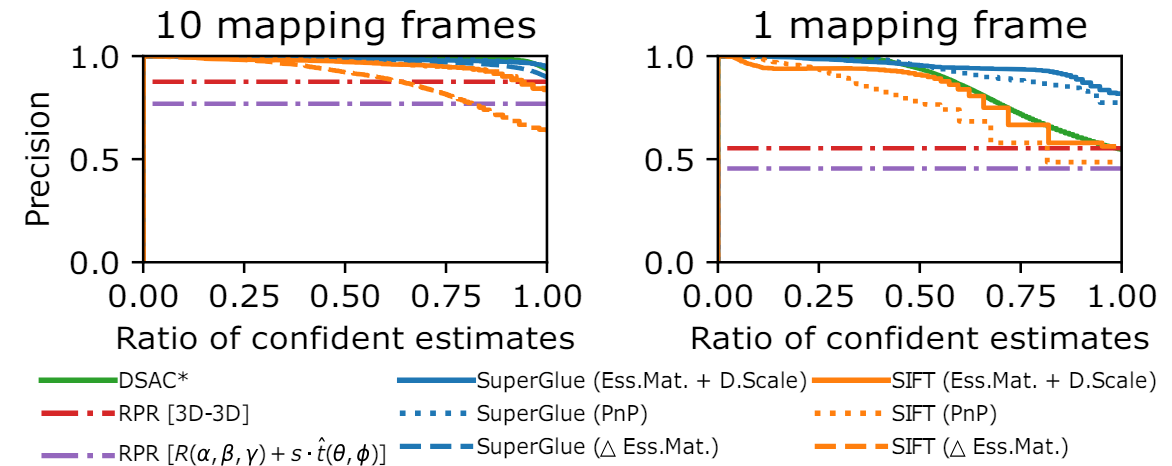
\includegraphics[width=0.6\textwidth]{pics/Proposal/partial_7scene.png}
  \caption[Hiệu quả của các mô hình khi giới hạn ảnh tham khảo]{Hiệu quả của những mô hình khi tập 7Scenes chỉ có 10/1 ảnh tham khảo, đánh giá về độ chính xác. Đối với những mô hình RPR không có phương pháp đánh giá về độ đáng tin cậy của dự đoán, một đường thẳng ngang sẽ được dùng để thể hiện độ chính xác}
\end{figure}

Để có thể phản ánh một môi trường thực tế, nơi mà ảnh tham khảo truy xuất được cách xa một khoảng đáng kể so với ảnh truy vấn, $K$ ảnh tham khảo mang nhiều thông tin nhất sẽ được chọn làm đại diện qua giải thuật gom cụm K-means.

Hai đồ thị trên thể hiện sự thay đổi về độ chính xác, những dự đoán có $VCRE<80px$ khi tỷ lệ kết quả chấp nhận thay đổi. Tỷ lệ số dự đoán chấp nhận sẽ tăng dần khi ngưỡng chấp nhận dần lỏng ra. Điều này đồng thời cũng làm cho độ chính xác cũng giảm dần do tăng khả năng những dự đoán không có cơ sở chắc chắn cũng được xem là đáng tin. Trong trường hợp này, những mô hình 2D-2D, đặc biệt là mô hình sử dụng SuperGlue, có kết quả tốt hơn so với những mô hình còn lại. Điều này thể hiện rõ nhất trong khoảng 0.5~1.0 ở cả 2 kịch bản $K=10$ và $K=1$.

Mô hình DSAC* vẫn có kết quả cạnh tranh. Tuy nhiên, phương pháp này lại quá phụ thuộc vào tập dữ liệu. Trong khi đó, những mô hình khác được huấn luyện trên tập ScanNet vẫn có kết quả tốt trên tập 7Scenes. Phương pháp sử dụng phép Triangulation cũng có kết quả cạnh tranh, tuy nhiên lại không thể hoạt động chỉ với một ảnh tham khảo. Những phương pháp Feat.Matching - Depth Scale có khả năng khái quát hóa tốt hơn những phương pháp RPR End-to-End, thể hiện qua hiệu quả tương đối tốt hơn.

\subsubsection{Tập dữ liệu Niantic}

\begin{figure}[H]
  \centering
  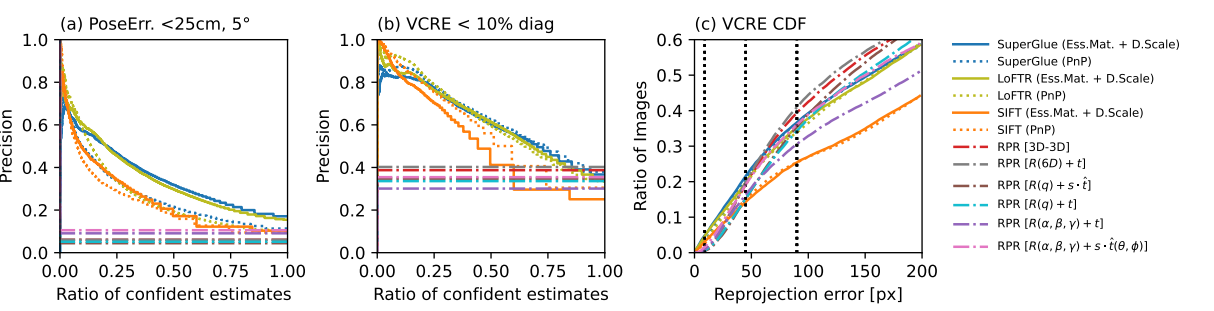
\includegraphics[width=\textwidth]{pics/Proposal/all_niantic.png}
  \caption{Hiệu quả của các mô hình trên tập dữ liệu Niantic, xác định theo độ chính xác và số ảnh có sai số phản chiếu dưới ngưỡng}
\end{figure}

Qua kết quả thu được, tập dữ liệu Niantic có độ khó cao hơn đáng kể so với tập dữ liệu 7Scenes với mọi phương pháp. Trong tập dữ liệu Niantic, những phương pháp Feat.Matching - Depth Scale tiếp tục có kết quả tốt. Tuy nhiên, ở những ngưỡng đáng tin cậy rộng hơn, những phương pháp RPR lại có kết quả tốt hơn. Điều này có thể giải thích được qua hiện tượng: khi số cặp đặc trưng tương quan là không đủ chất lượng, độ lệch đơn vị vị trí được sinh ra có sai số rất lớn so với thực tế ở những phương pháp Feat.Matching - Depth Scale. Những phương pháp RPR End-to-End cho ra kết quả tốt khi ngưỡng chính xác rộng, nhưng lại có kết quả không tốt khi cần độ chính xác cao. Ngoài ra, những phương pháp RPR End-to-End cũng không thể cung cấp độ tin cậy cho dự đoán của mô hình, không thể loại bỏ những dự đoán có khả năng sai cao.

\section{Đề xuất phát triển}

\subsection{Chiến lược khai phá đặc trưng dựa trên độ trùng lắp}
Ảnh tham khảo truy xuất được từ tác vụ VPR tiềm ẩn rủi ro không đủ độ trùng lắp với ảnh đầu vào, dẫn đến sai sót trong quá trình tính toán tư thế. Để giải quyết vấn đề này, chúng tôi đề xuất một chiến lược khai phá mới dựa trên hàm khai phá Multi-Similarity Miner \cite{wang2019multi} nhằm đảm bảo tính trùng lấp về vùng khung hình(frustum) cao giữa các ảnh. Điều này sẽ hỗ trợ cho quá trình Feature Matching tại module RPR ở phía sau.

Cụ thể hơn, chúng tôi xác định một cặp ảnh là được một positive pair nếu có độ trùng lắp frustum cao hơn một ngưỡng nhất định, tức giữa cặp ảnh chia sẻ nhiều điểm chung hơn. Để đảm bảo độ vững chắc của mô hình không bị tác động, chúng tôi sử dụng cơ chế trùng lắp camera frustum song phương từ \cite{9008579}, được tính bằng tổng độ trùng lắp frustum từ một ảnh đến ảnh còn lại và ngược lại.

Tuy nhiên, độ trùng lắp cao vẫn có thể xuất hiện trong trường hợp các ảnh được chụp ở hai góc độ hoàn toàn ngược nhau, gây nên khó khăn và sai lệch trong quá trình dự đoán tư thế tuyệt đối do góc quay khác biệt quá lớn. Để giải quyết vấn đề này, chúng tôi đặt ra điều kiện khác biệt hướng nhìn làm một tiêu chuẩn phụ trong việc chấp nhận các cặp ảnh. Cụ thể hơn, các cặp ảnh không được phép có hướng nhìn lệch nhau quá một tiêu chuẩn nhất định mà chúng tôi đặt ra.

% \begin{figure}
%   \centering
%   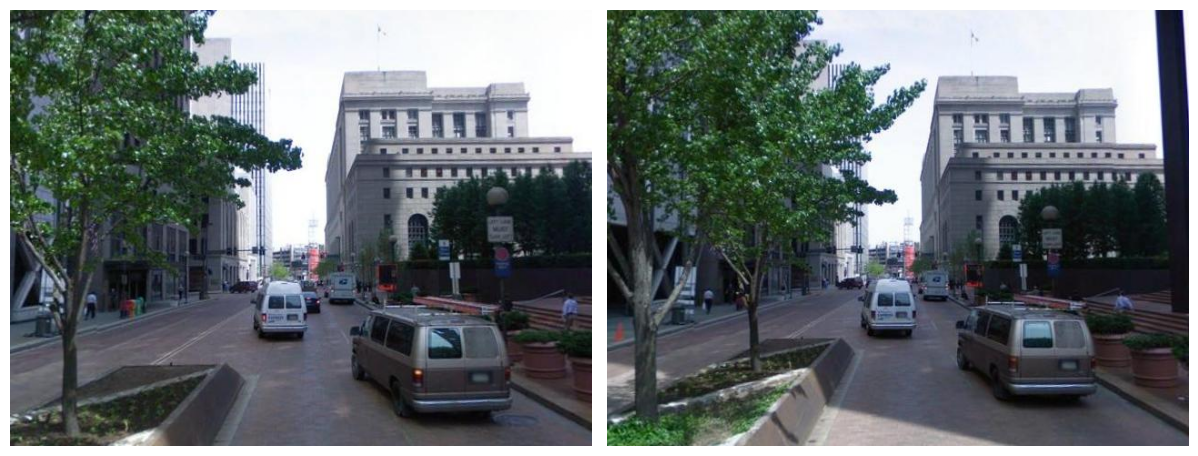
\includegraphics[width=\textwidth]{pics/Chapter3/highoverlap.png}
%   \caption[Cặp ảnh có độ overlap cao]{Cặp ảnh được chấp nhận - có độ trùng lắp cao}
% \end{figure}

% \begin{figure}
%   \centering
%   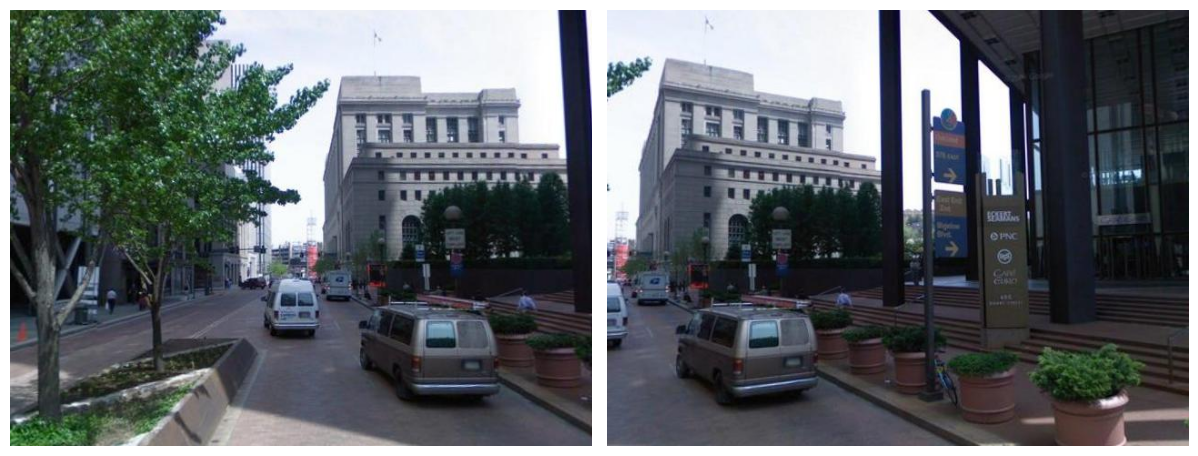
\includegraphics[width=\textwidth]{pics/Chapter3/lowoverlap.png}
%   \caption[Cặp ảnh có độ overlap thấp]{Cặp ảnh không được chấp nhận - có độ trùng lắp thấp}
% \end{figure}

\begin{figure}
  \centering
  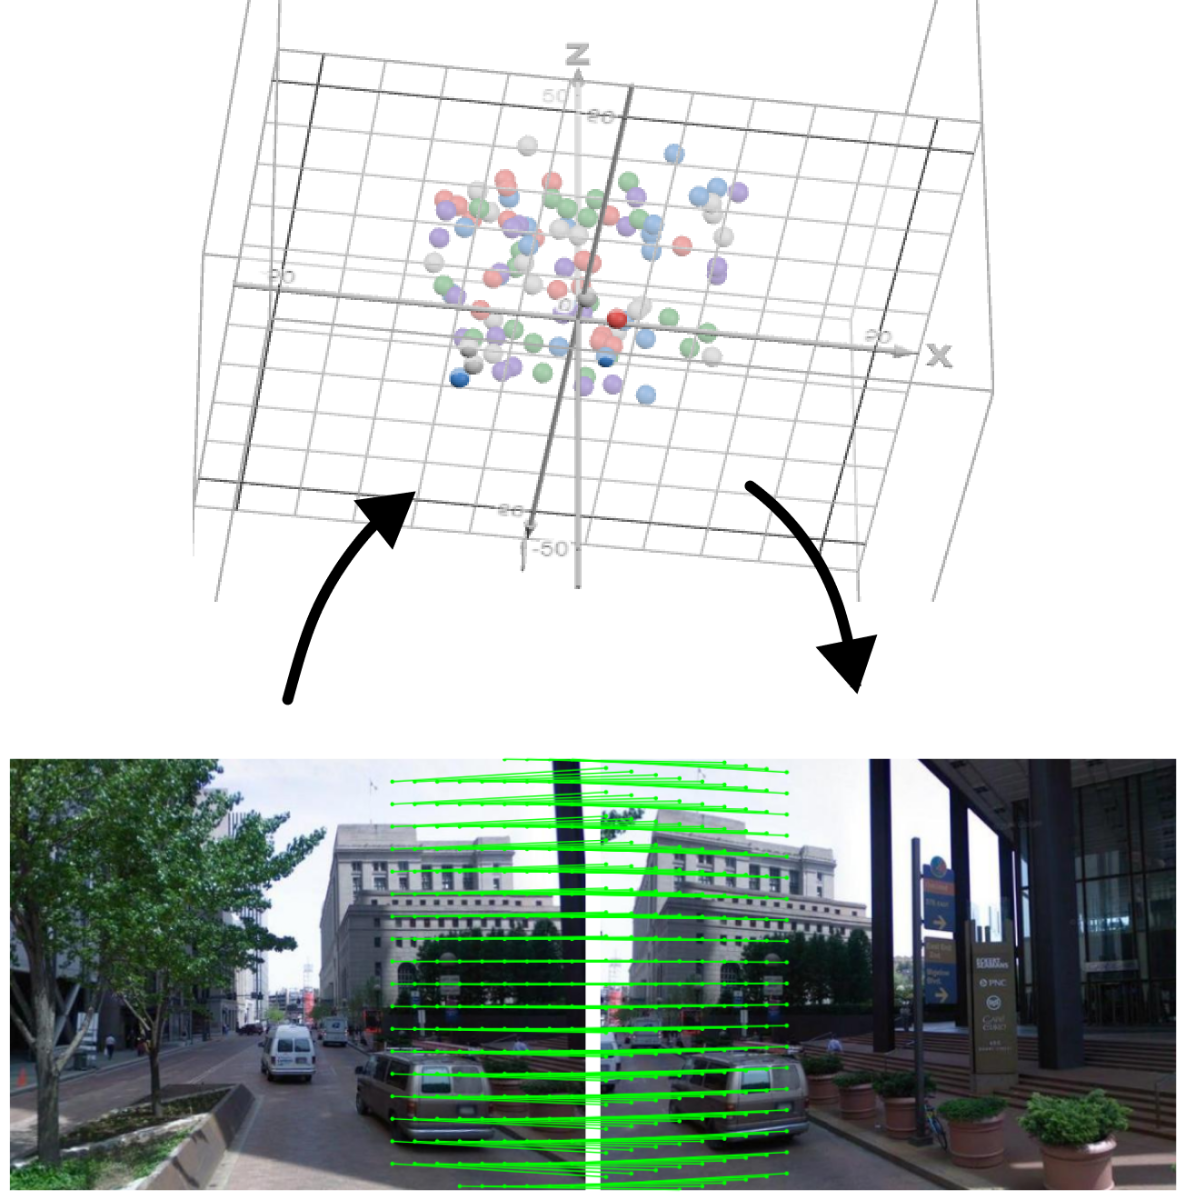
\includegraphics[width=\textwidth]{pics/Proposal/project.drawio.png}
  \caption[Quá trình chiếu giữa 2 ảnh]{Ảnh mô tả quá trình chiếu từ ảnh đầu tiên lên không gian 3D rồi back-project lên không gian khung hình của ảnh thứ 2}
\end{figure}

\subsubsection*{Độ trùng lắp Frustum}

Độ trùng lắp frustum giữa hai ảnh có thể được định nghĩa là tổng tỷ lệ các điểm ảnh thuộc ảnh thứ nhất nằm trong vùng tầm nhìn khi chiếu lên hệ tọa độ camera thứ hai, và ngược lại. Độ trùng lắp này được tính toán bằng cách trước hết chiếu các điểm ảnh từ hình ảnh gốc vào không gian 3D thông qua việc tận dụng độ sâu ước lượng được. Sau đó, các điểm ảnh này được chiếu vào hệ tọa độ của hình ảnh thứ hai bằng cách tận dụng thông tin vị trí và góc quay của chúng.

Đầu tiên, một ma trận các điểm ảnh với kích thước 10x10 được chiếu vào hệ tọa độ thực, sau đó lại được chiếu lại vào hệ tọa độ camera thứ hai. Phép chiếu có thể được công thức hóa như sau:
$$
W = R_1\cdot \left[(K_1^{-1} \cdot P_1)*D_1(P_1)\right] + t_1
$$

$$
P_2 = K_2 \cdot\left[R_2^{T} \cdot (W - t_2)\right]
$$
với $P_i$ là vị trí điểm ảnh trong camera $i$, $K_i$ là ma trận intrinsics, $R_i$ và $t_i$ là độ lệch góc quay và vị trí từ hệ tọa độ camera sang hệ tọa độ thực với $R$ là vector góc quay thu được từ quaternion tương ứng, và $D_i(P)$ là ước lượng độ sâu theo đơn vị khoảng cách của điểm ảnh $P$.

\subsubsection*{Khác biệt hướng nhìn}

Để kiểm soát cách biệt góc quay giữa hai ảnh, chúng tôi đo độ cách biệt về hướng nhìn giữa chúng. Độ lệch góc quay camera $\alpha$ giữa hai camera có thể được định nghĩa như sau:

$$
\alpha = arccos\left(\frac{trace(R_1^T \cdot R_2 - 1)}{2} \right) / \pi * 180
$$

với $\alpha$ mang đơn vị độ và $R_i$ là ma trận 3x3 thể hiện góc quay của ảnh.

\subsubsection*{Hàm Loss}

Hàm loss của chúng tôi được tính toán bằng tổng có trọng số giữa hai hàm loss với một biến số 'Control Rate' - tỷ lệ kiểm soát:
$$
L = \beta * L_{Miner} + (1-\beta)*L_{Control}
$$
với $L_{Control}$ là hàm Multi-Similarity Loss từ bài báo Multi-Similarity Miner và $L_{Miner}$ là hàm Multi-Similarity Loss nhận đầu ra từ chiến lược khai phá frustum mới của chúng tôi và $\beta$ là giá trị tỷ lệ để kiểm soát hai hàm Loss trên.

\subsection{Chiến lược sắp xếp lại ảnh}
Một số nghiên cứu trước đây đã thiết kế tác vụ truy xuất ảnh ở module VPR thành một quá trình gồm 2 bước đi từ kết quả thô đến kết quả chính xác. Việc thực hiện quá trình 2 bước này giúp cho mô hình VPR có thể lọc được tập kết quả thô ban đầu và sau đó tinh chỉnh lại xếp hạng của các kết quả theo một tiêu chí khác. Trong phương pháp đề xuất của chúng tôi, bước truy xuất đầu tiên sẽ được dùng để xác định một tập $k_1$ các ảnh được chụp gần với ảnh truy vấn. Sau đó, bước sắp xếp lại phía sau sẽ sắp xếp lại thứ tự ảnh, sắp xếp theo ưu tiên những ảnh có độ trùng lấp cao với ảnh truy vấn và xác định top $k_2$ ảnh có độ trùng lấp cao nhất.

Với bước truy xuất ban đầu, chúng tôi sử dụng trọng số baseline được cung cấp bởi mô hình MixVPR, do đã được chứng minh là có hiệu quả tốt trong việc xác định ảnh tham khảo có vị trí gần với ảnh truy vấn. Sau đó, ở bước sắp xếp lại thứ tự, chúng tôi sử dụng một trọng số khác của MixVPR đã được huấn luyện lại, tập trung vào việc xác định những ảnh có độ trùng lấp cao với nhau. 

Để có được trọng số mới, chúng tôi huấn luyện mô hình trên tập dữ liệu GSV-Cities \cite{Ali_bey_2022} với mỗi batch sẽ chỉ gồm các ảnh từ 1 khu vực. Mô hình sẽ tập trung vào việc phân biệt những ảnh có độ trùng lấp khung hình cao và thấp theo tiêu chí đã được đặt ra ở \textbf{3.4.1}.

\begin{figure}
  \centering
  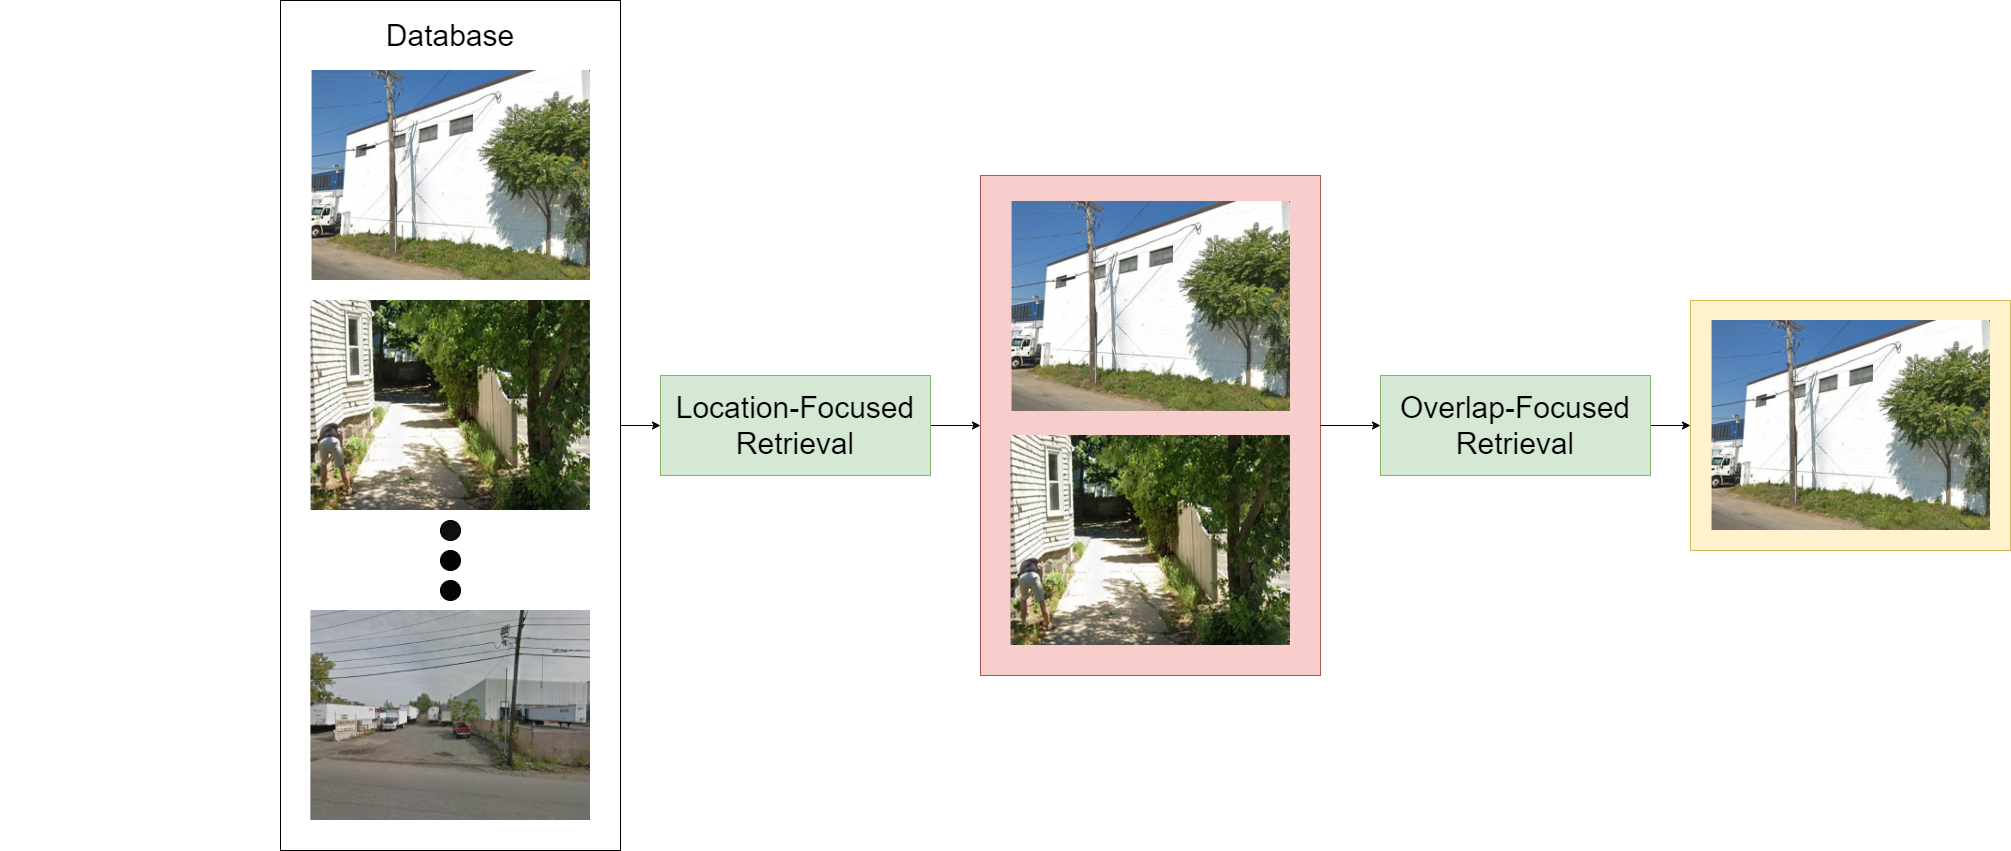
\includegraphics[width=\textwidth]{pics/Proposal/rerank.drawio.png}
  \caption[Quá trình truy xuất 2 bước của VPR]{Quá trình truy xuất gồm 2 bước của mô hình VPR, gồm truy xuất theo địa điểm và truy xuất theo độ trùng lắp}
\end{figure}

\subsection{Trung bình trọng số của các dự đoán}

Ở pipeline cơ bản được đề xuất của nhóm, module VPR sẽ truy xuất được $k$ ảnh tham khảo và từ đó có thể xác định được $k$ dự đoán khác nhau tương ứng với mỗi ảnh. Kết quả cuối cùng sẽ là dự đoán có độ đáng tin cậy $C$ cao nhất. Tuy nhiên, khi chọn theo cơ chế tối đa như thế, thông tin lấy được từ những dự đoán của những ảnh còn lại sẽ bị lãng phí. Vì vậy nên, chúng tôi giới thiệu phương pháp lấy trung bình của từng dự đoán dựa vào với trọng số tương ứng với độ đáng tin $C$.

\begin{figure}[H]
  \centering
  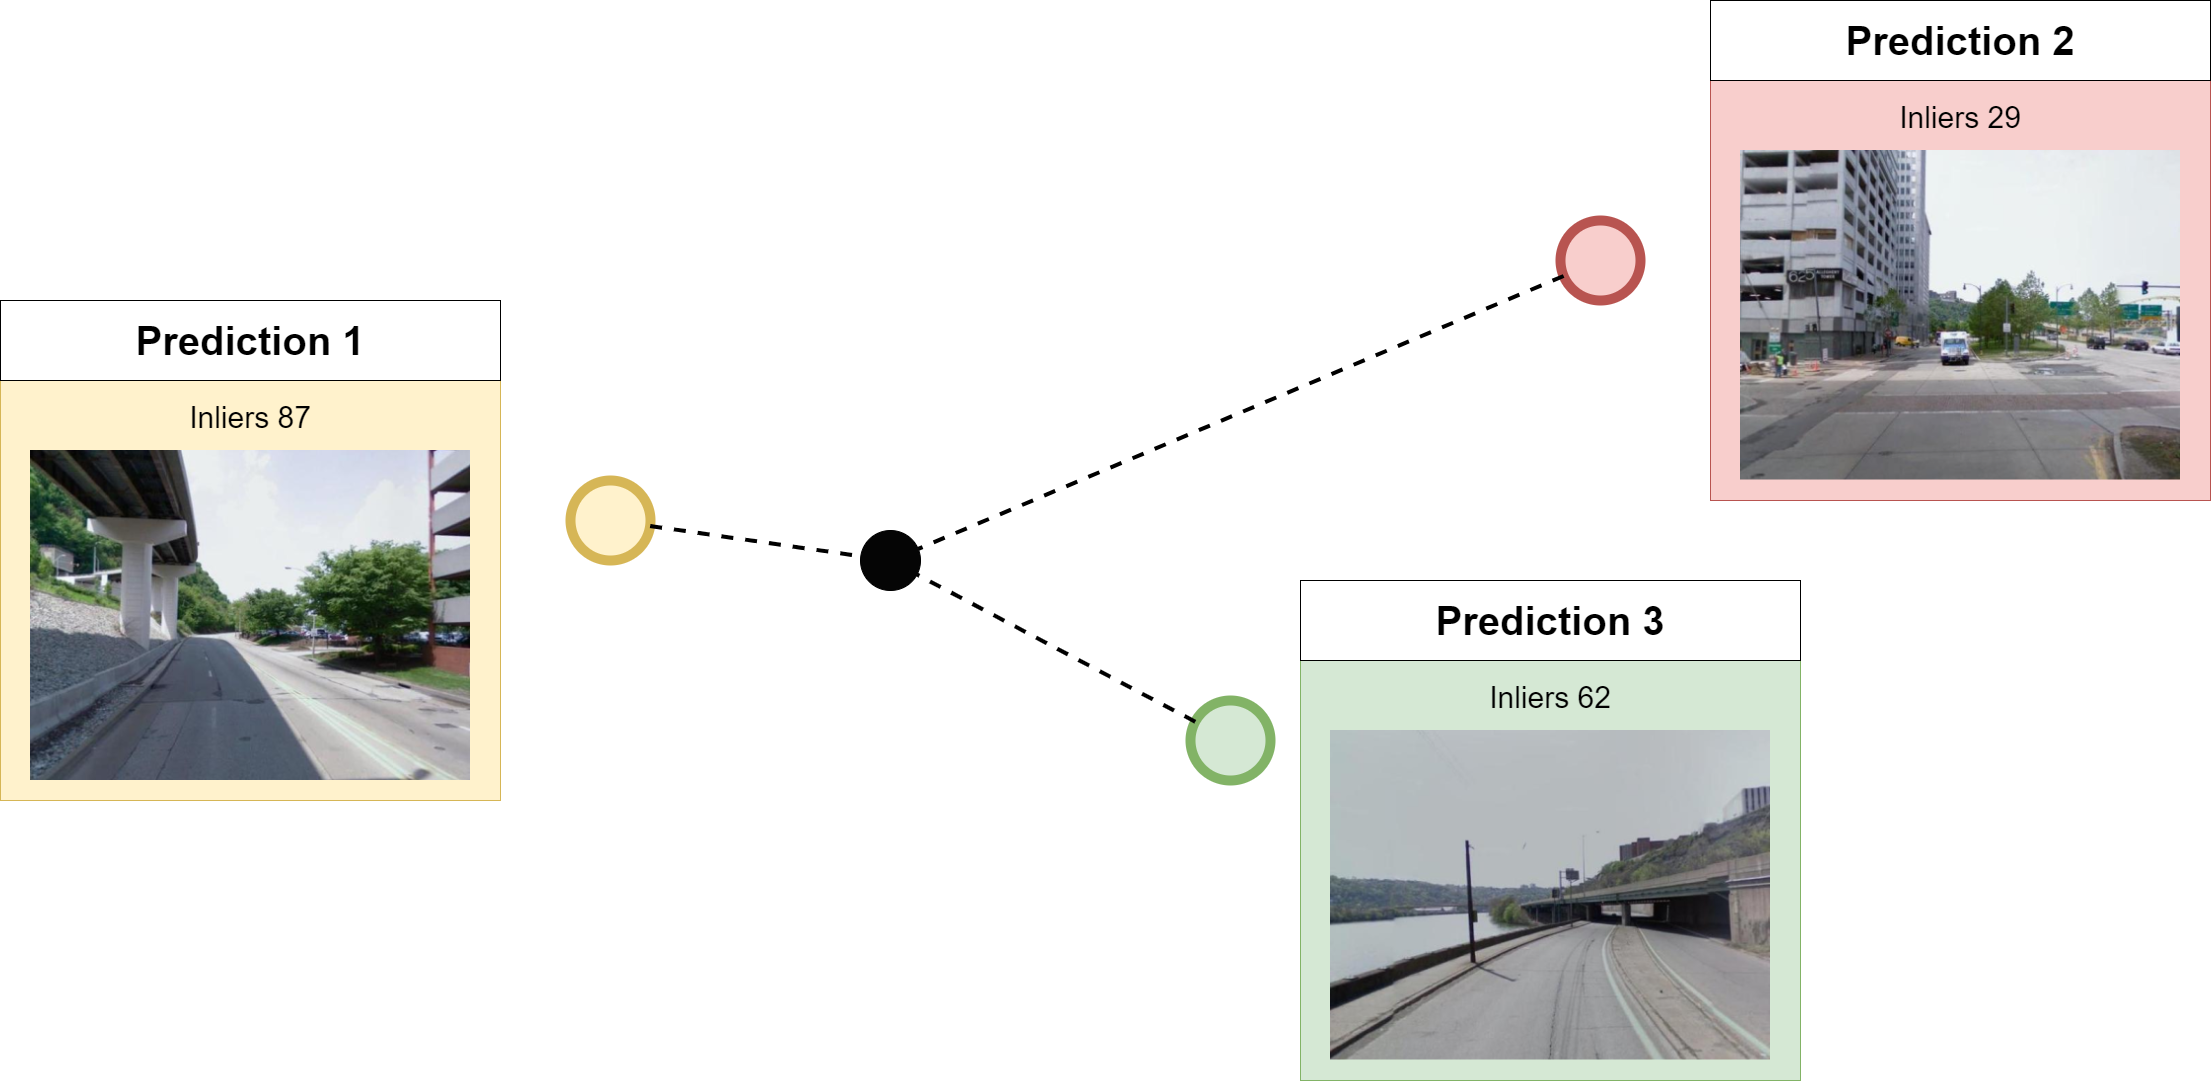
\includegraphics[width=\textwidth]{pics/Proposal/weighted.png}
  \caption[Trung bình trọng số theo inliers của dự đoán]{Mô tả phương pháp lấy trung bình trọng số của các dự đoán theo độ tin cậy của dự đoán}
\end{figure}

\subsection{Giới hạn ngưỡng đáng tin của kết quả}

Độ đáng tin cậy $C$ của dự đoán của cặp ảnh truy vấn và tham khảo được định nghĩa là số cặp điểm tương quan giữa hai hình mà khi áp dụng phép biến đổi tương ứng với độ lệch về tư thế giữa hai ảnh, cho ra độ lệch dưới một ngưỡng nhất định. Càng nhiều điểm thỏa được phép biến đổi thì cơ sở để suy luận ra được độ lệch giữa hai ảnh càng thêm chắc chắn. Vì vậy nên, để đảm bảo được dự đoán của pipeline có thể được tin tưởng, chúng tôi áp dụng một bước lọc lại dự đoán ở cuối pipeline, nhằm lọc ra những kết quả có độ đáng tin cậy thấp, từ đó cải thiện hiệu quả của mô hình.

\begin{figure}[H]
  \centering
  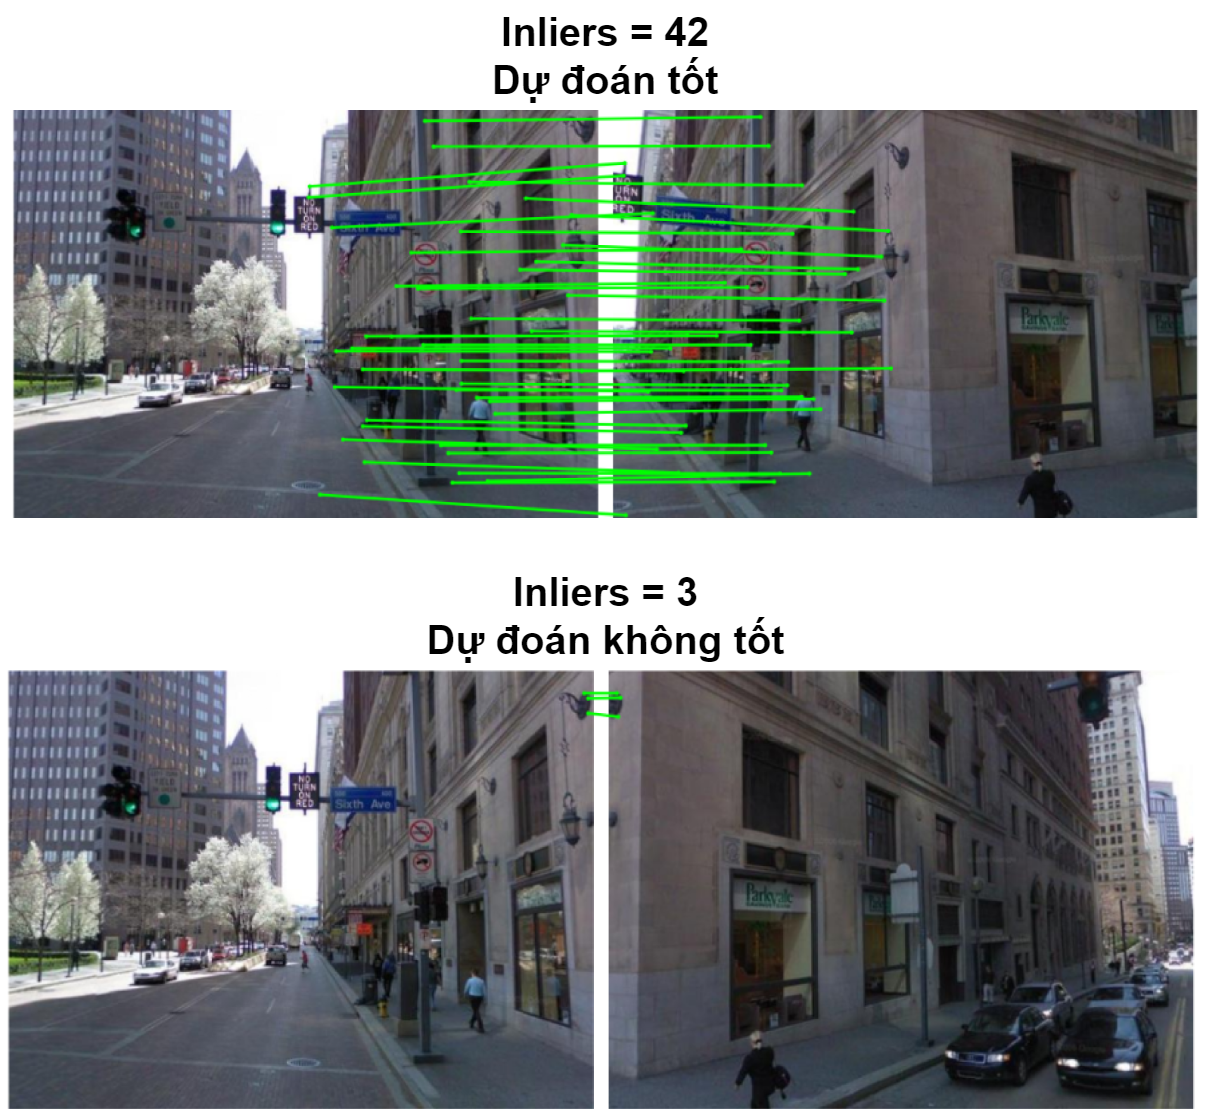
\includegraphics[width=\textwidth]{pics/Proposal/threshold.png}
  \caption[Những dự đoán tốt và không tốt đánh giá theo độ tin cậy]{Mô tả những trường hợp có độ tự tin cao và thấp trong tập dữ liệu Pittsburgh250k \cite{6618963}}
\end{figure}

